\documentclass[12pt,a4paper,twoside]{book}
\usepackage{graphicx}
\usepackage{setspace}	%double spacing for text, single for captions, footnotes, etc.
%\usepackage{hypernat} 	%substitut de cite que permet fer hyperlinks
\usepackage{natbib}		% substituye a 'hypernat' que funciona en Windows.
\usepackage[spanish]{babel}
\usepackage[utf8]{inputenc}
\usepackage{color}
\usepackage{hhline} 		% extended styles for tables
\usepackage{multirow}
\usepackage{subfigure}
\usepackage{acronym}
\usepackage{hyperref}
\usepackage{amsmath,amsmath,amssymb} 
\usepackage{fancyhdr}
\usepackage{epsfig, amsmath}
\usepackage{algorithm}
\usepackage{algorithmic}

% general settings
\hypersetup{
	linktocpage=true,
	colorlinks=true,
	linkcolor=blue,
	citecolor=blue,
}
\definecolor{Hgray}{gray}{0.6}

\newenvironment{definition}[1][Definition]{\begin{trivlist}
\item[\hskip \labelsep {\bfseries #1}]}{\end{trivlist}}

\setlength{\topmargin}{0cm}
\setlength{\textheight}{23cm}
\setlength{\textwidth}{17cm}
\setlength{\oddsidemargin}{0cm}
\setlength{\evensidemargin}{0cm}
\setlength{\headheight}{1cm}

% indica que las 'sub-sub-sections' sean numeradas y aparezcan en el indice
\setcounter{secnumdepth}{3}
\setcounter{tocdepth}{2}

% settings for code
\renewcommand{\algorithmicrequire}{\textbf{Entrada: }}
\renewcommand{\algorithmicensure}{\textbf{Salida: }}

%%%%%%%%%%%%
% DOCUMENT %
%%%%%%%%%%%%
\begin{document}

% portada
\newpage
\thispagestyle{empty}

\baselineskip 2em

%\vspace*{1cm}

\centerline{
\includegraphics[width=0.6\textwidth]{images/UOC-logo}}
\begin{center}
\textsc{Universitat Oberta de Catalunya (UOC) \\
 Máster Universitario en Ciencia de Datos (\textit{Data Science})\\}

%\centerline {\pic{UOC}{4cm}}

\vspace*{1.5cm}

\textsc{\Large TRABAJO FINAL DE MÁSTER}

\vspace*{0.5cm}

\textsc{\large Área: Informática, Multimedia y Telecomunicación}


%\textbf{\Huge VirtualTechLab Model: }

\vspace*{2.0cm}

\textbf{\Large Predicción de Panel Attrition con Machine Learning: El caso de la Encuesta Financiera de las Familias}

\textbf{\large }

\vspace{2.5cm}
\baselineskip 1em

\baselineskip 2em
-----------------------------------------------------------------------------\\
Autor:      Carlos Luis Gento de Celis\\
Tutor:      Jordi Escayola Mansilla\\
Profesor:   Ismael Benito Altamirano\\
-----------------------------------------------------------------------------\\
\vspace*{1.5cm}
Madrid, \today

\end{center}

\newpage
\pagestyle{empty}
\hfill

\newpage
% abstract
\pagenumbering{roman} 
\setcounter{page}{1} 
\pagestyle{plain}

%%%%%%%%%%%%%%%%
%%% CREDITOS %%%
%%%%%%%%%%%%%%%%
\chapter*{Créditos/Copyright}

\vspace{1cm}

\begin{figure}[ht]
    \centering
	
\includegraphics[scale=1]{images/license.png}
\end{figure}

Esta obra está sujeta a una licencia de Reconocimiento -  NoComercial - SinObraDerivada

\href{https://creativecommons.org/licenses/by-nc-nd/3.0/es/}{3.0 España de CreativeCommons}.

%%%%%%%%%%%%%
%%% FICHA %%%
%%%%%%%%%%%%%
\chapter*{FICHA DEL TRABAJO FINAL}

\begin{table}[ht]
	\centering{}
	\renewcommand{\arraystretch}{2}
	\begin{tabular}{r | p{10cm}}
		\hline
		Título del trabajo: & Predecir panel attrition con Machine Learning: Un análisis con la Encuesta Financiera de las Familias\\
		\hline
        Nombre del autor: & Carlos Luis Gento de Celis\\
		\hline
        Nombre del colaborador/a docente: & Jordi Escayola Mansilla\\
		\hline
        Nombre del PRA: & Antonio Lozano Bagén\\
		\hline
        Fecha de entrega (mm/aaaa): & 10/2023\\
		\hline
        Titulación o programa: & Máster Universitario en Ciencia de Datos\\
		\hline
        Área del Trabajo Final: & Informática, Multimedia y Telecomunicación\\
		\hline
        Idioma del trabajo: & Español\\
		\hline
        Palabras clave & predictive models, machine learning, panel attrition\\
		\hline
	\end{tabular}
\end{table}

%%%%%%%%%%%%%%%%
%%% RESUMEN  %%%
%%%%%%%%%%%%%%%%

\chapter*{Resumen}
\addcontentsline{toc}{chapter}{Resumen}

\onehalfspacing

La Encuesta Financiera de las Familias (EFF) es una encuesta bienal cuyo objetivo es recoger información sobre la situación económico-financiera de los hogares que residen en España, y su evolución a lo largo del tiempo. Para ello, los hogares seleccionados pueden participar en hasta cuatro olas consecutivas de la encuesta. Sin embargo, hay hogares que abandonan el estudio antes de tiempo. Aunque estos abandonos no interrumpan el estudio, sí podrían afectar a sus resultados si el número de abandonos es demasiado grande, o si se concentra en colectivos específicos de la población. Es importante analizar las causas de estos abandonos y desarrollar herramientas que puedan evitarlos.

Este documento, en primer lugar, analiza las características de los hogares que participaron en la Encuesta Financiera de las Familias (EFF) en sus ediciones de 2017 y 2020, y si participaron en las olas de 2020 y de 2022. A continuación, plantea una serie modelos de predicción basados en métodos de Machine Learning y evalúa su capacidad para predecir si un hogar abandonará la EFF en 2020 o en 2022. Finalmente, interpreta los resultados el modelo que mejor ha funcionado.

\vspace{1.5cm}

\textbf{Palabras clave}: predictive models, panel attrition, machine learning, household surveys

\chapter*{Abstract}
\addcontentsline{toc}{chapter}{Abstract}

\onehalfspacing

The Spanish Survey of Household Finances (EFF) is a biennial survey whose goal is to collect information about the economical and financial situation of households in Spain, and its evolution through time. To do so, selected households may take part in up to four consecutive waves of this survey. However, some households cease their participation prematurely. Although withdrawals do not interrupt the research study, they might affect its results if the number of withdrawals is too high, or if it is more likely to happen for certain groups of people. It is important to analyse the causes of this phenomenon and develop tools to prevent it.

Firstly, this paper analyses the characteristics of households that responded to the EFF in its editions of 2017 and 2020, and their participation during the 2020 or 2022 waves. Next, a series of predictive models based on machine learning methods are considered and evaluated for the exercise of predicting panel attrition in the EFF. Finally, it interprets the results of the most successful model.

\vspace{1.5cm}

\textbf{Key words}: predictive models, panel attrition, machine learning, longitudinal surveys, household surveys
\newpage

\pagestyle{fancy}
\renewcommand{\chaptermark}[1]{ \markboth{#1}{}}
\renewcommand{\sectionmark}[1]{\markright{ \thesection.\ #1}}
\lhead[\fancyplain{}{\bfseries\thepage}]{\fancyplain{}{\bfseries\rightmark}}
\rhead[\fancyplain{}{\bfseries\leftmark}]{\fancyplain{}{\bfseries\thepage}}
\cfoot{}

% indice
\cleardoublepage
\phantomsection
\addcontentsline{toc}{chapter}{Índice}
\tableofcontents

\thispagestyle{empty}

\pagenumbering{arabic}

\pagestyle{fancy}
\renewcommand{\chaptermark}[1]{ \markboth{#1}{}}
\renewcommand{\sectionmark}[1]{\markright{ \thesection.\ #1}}
\lhead[\fancyplain{}{\bfseries\thepage}]{\fancyplain{}{\bfseries\rightmark}}
\rhead[\fancyplain{}{\bfseries\leftmark}]{\fancyplain{}{\bfseries\thepage}}
\cfoot{}

\onehalfspacing

% capitulos del documento
\chapter{Introducción}
\label{chapter:introduccion}

Los estudios longitudinales son proyectos de investigación en los que se hace un seguimiento a un grupo de unidades muestrales (personas, hogares...) a lo largo de un período de tiempo. En el ámbito de las ciencias sociales, la recolección de datos de muchos de estos estudios se realiza mediante el uso de encuestas, de tal manera que las mismas personas responden a las preguntas del mismo cuestionario de manera repetida durante un tiempo, que pueden ser semanas, meses o incluso años. Esto da lugar a las llamadas encuestas longitudinales o encuestas panel. La dimensión temporal de estas encuestas las convierten en una herramienta muy útil para poder analizar relaciones causales, ya que permiten observar cambios en opiniones, comportamientos o estados de los mismos panelistas a lo largo del tiempo. Sin embargo, la calidad de esos análisis depende de la cooperación exitosa y continuada de dichos panelistas durante las sucesivas ediciones u olas de la encuesta. El abandono prematuro y acumulado en el tiempo de participantes en un panel se conoce como \textbf{Panel Attrition} (\cite{watson2009identifying}).

\cite{lynn2018tackling} destaca que el Panel Attrition presenta dos principales problemas. Por un lado, si la tasa de abandonos es alta, el tamaño de la muestra se reducirá drásticamente en pocas olas, lo que provocará que la precisión de los estimadores de la encuesta sea muy baja, y además limitará o incluso imposibilitará el análisis de subgrupos dentro de la muestra. Por otro lado, si el Panel Attrition no es aleatorio y los panelistas que abandonan la encuesta son sistemáticamente diferentes a los que se mantienen, existe el riesgo de introducir un sesgo de no-respuesta en los estimadores de la encuesta.

Tradicionalmente, los métodos utilizados para mitigar los efectos del Panel Attrition se han centrado en el impacto estadístico que provoca, principalmente con el uso de métodos de imputación múltiple (\cite{rubin1987multiple}), la reponderación de pesos muestrales (\cite{groves2009survey}) e introduciendo muestras de refresco para sustituir a las unidades muestrales perdidas (\cite{hirano1998combining}). Pero en las últimas décadas ha aumentado el interés por tratarlo durante los procesos de creación y recolección de datos, lo que ha llevado a la extensión del uso de los llamados diseños adaptativos y reactivos (adaptative and responsive designs, \cite{tourangeau2017adaptive}). La idea detrás de estos diseños se fundamenta en utilizar toda la información que se genera durante la elaboración de encuestas (respuestas al cuestionario, paradata u observaciones de los entrevistadores) para diseñar implementaciones informadas cuyo objetivo sea mejorar la calidad de los datos, reducir los costes, o ambos. En este sentido, las encuestas longitudinales ofrecen una gran oportunidad para estos diseños porque contienen mucha información tanto de los trabajos de campo que se estén desarrollando, como los que se realizaron en olas anteriores. Por ejemplo, se ha utilizado información sobre intentos de contacto en olas pasadas para revisar la estrategia de incentivos para hogares a los que cuesta volver a entrevistar (\cite{mcgonagle2022effects}) o para optimizar las estrategias de contacto en las ediciones siguientes (\cite{kreuter2015note}).

Dentro de este contexto de los diseños adaptativos y reactivos, en las últimas décadas se ha desarrollado el uso algoritmos de Machine Learning en la metodología de encuestas, especialmente para predecir Panel Attrition (\cite{buskirk2018introduction}). Por ejemplo, en \cite{beste2023case} utilizan información de ediciones pasadas de una encuesta a hogares en Alemania para entrenar varios modelos basados en algoritmos de Machine Learning para identificar hogares panelistas con una baja probabilidad de volver a participar en la siguiente edición. Posteriormente, utilizan el mejor de esos modelos para predecir cuáles hogares panelistas de una nueva edición tenían menor probabilidad de colaborar de nuevo, y usan esas predicciones para crear un diseño experimental enfocado en esos hogares.

El objetivo de este Trabajo de Fin de Máster es adaptar la implementación de Machine Learning vista en \cite{beste2023case} para predecir la participación de los hogares panel al caso de estudio de la Encuesta Financiera de las Familias (EFF). La EFF es una encuesta a hogares representativa de los hogares que residen en España, y es creada por el Banco de España. La idea central del ejercicio de predicción consiste en utilizar información de hogares en olas pasadas de la EFF para predecir una variable binaria de participación o no participación en la ola siguiente. Para ello, se entrenan cuatro modelos basados en algoritmos de Machine Learning y se compara su rendimiento con un modelo de referencia utilizado tradicionalmente en análisis de Panel Attrition, que en este caso es una Regresión Logística o Logit. En este proyecto, para el entrenamiento de los modelos se utiliza información sobre hogares que han participado en las olas 4, 5, 6 y 7 de la EFF (que se corresponden con los años 2011, 2014, 2017 y 2020), y a continuación se utilizan dichos modelos para predecir la participación de los hogares panel elegibles para la ola 8 (que se corresponde con el año 2022).

Los seis capítulos restantes de este documento se organizan de la siguiente manera. En el siguiente capítulo se exponen los objetivos, la planificación del proyecto y las motivaciones personales para realizarlo. En el tercer capítulo se hace una revisión del estado del arte para este estudio, en el que se describe cuáles son las causas del Panel Attrition, cómo se están utilizado algoritmos de Machine Learning para predecirlo, y finalmente se presenta la Encuesta Financiera de las Familias (EFF). En el cuarto capítulo se describe la metodología utilizada en el análisis exploratorio de datos y en el ejercicio de entrenamiento, validación y test de los modelos de predicción de Panel Attrition. En el quinto capítulo se presentan los datos de la EFF y se realizan una descripción de las etapas de producción de la EFF, y un análisis exploratorio de los datos. En el sexto capítulo se muestran y comentan los resultados del entrenamiento y la evaluación de los modelos de predicción, y se analiza la importancia de las variables utilizadas en uno de los modelos de predicción para explicar el Panel Attrition. Finalmente, en el último capítulo se exponen las conclusiones y reflexiones sobre el proyecto y cuáles pueden ser las líneas de trabajo para el futuro.
\chapter{Objetivos del proyecto, planificación y motivación personal}
\label{chapter:objetivos}
\section{Objetivos del proyecto}

Este proyecto se contextualiza dentro del marco de la metodología de encuestas. En concreto, se centra en las encuestas longitudinales a hogares, y dentro de ese campo pone el foco en la predicción de la participación de los hogares en olas posteriores a su primera colaboración. La encuesta elegida para el proyecto es la Encuesta Financiera de las Familias (EFF), una encuesta de referencia para investigaciones sobre finanzas de los hogares.

El \textbf{objetivo principal} de este proyecto es desarrollar un modelo de predicción basado en métodos de machine learning que ayude a predecir si un hogar que ha participado en al menos una ola de la EFF volverá a hacerlo en olas posteriores.

Para poder desarrollar ese modelo, es necesario completar una serie de \textbf{objetivos secundarios}. Estos objetivos se agruparán en 5 fases:

\begin{enumerate}[noitemsep]
    \item Hacer una revisión del estado del arte sobre el Panel Attrition y las metodologías de Machine Learning aplicadas a su predicción.
    \item Recolección de datos. Preferentemente, obtener un conjunto de datos que contenga:
    \begin{enumerate}
        \item Las respuestas de los hogares al cuestionario de la EFF.
        \item Paradata sobre el proceso de creación de la encuesta.
        \item Características de los entrevistadores.
    \end{enumerate}
    \item Análisis exploratorio de los datos. Identificar patrones dentro de los datos que puedan estar relacionados con el panel attrition.
    \item Preprocesar los datos para entrenar modelos de machine learning.
    \item Modelado y evaluación de modelos de predicción basados en métodos de machine learning.
    \item Interpretación del mejor modelo y redacción de conclusiones.
\end{enumerate}

\section{Planificación del proyecto}

La planificación de este proyecto se va a dividir en 5 fases. La asignación temporal a cada una de ellas se ha realizado de acuerdo a la estructura de contenidos del Plan Docente y al calendario de la asginatura.

\begin{enumerate}[noitemsep]
    \item Fase 1: Contiene la definición del proyecto y la planificación del TFM. Abarca las dos primeras semanas del proyecto, del 27 de septiembre al 10 de octubre.
    \item Fase 2: Contiene las tareas de la revisión de la literatura y la caracterización del panel attrition de la EFF. Abarcará desde el 11 de octubre al 23 de octubre.
    \item Fase 3: Contiene las tareas de recolección de datos, análisis exploratorio de dichos datos, preprocesamiento para entrenar los modelos de machine learning, modelado y evaluación de los modelos de predicción, y la interpretación de los modelos y la redacción de conclusiones. Esta fase es la más duradera y abarcará desde el 17 de octubre al 19 de diciembre.
    \item Fase 4: En esta fase se procederá a la redacción de la memoria del TFM y la preparación de una presentación audiovisual sobre el proyecto. Abarcará desde el 20 de diciembre al 18 de enero.
    \item Fase 5: En esta fase final se procederá a la defensa del TFM. Esa etapa abarcará desde el 22 de enero hasta el 4 de febrero.
\end{enumerate}

 En la figura \ref{fig:gantt} puede observarse la distribución temporal y el tiempo dedicado a cada tarea en un diagrama de Gantt.


\begin{figure}
	\centering
	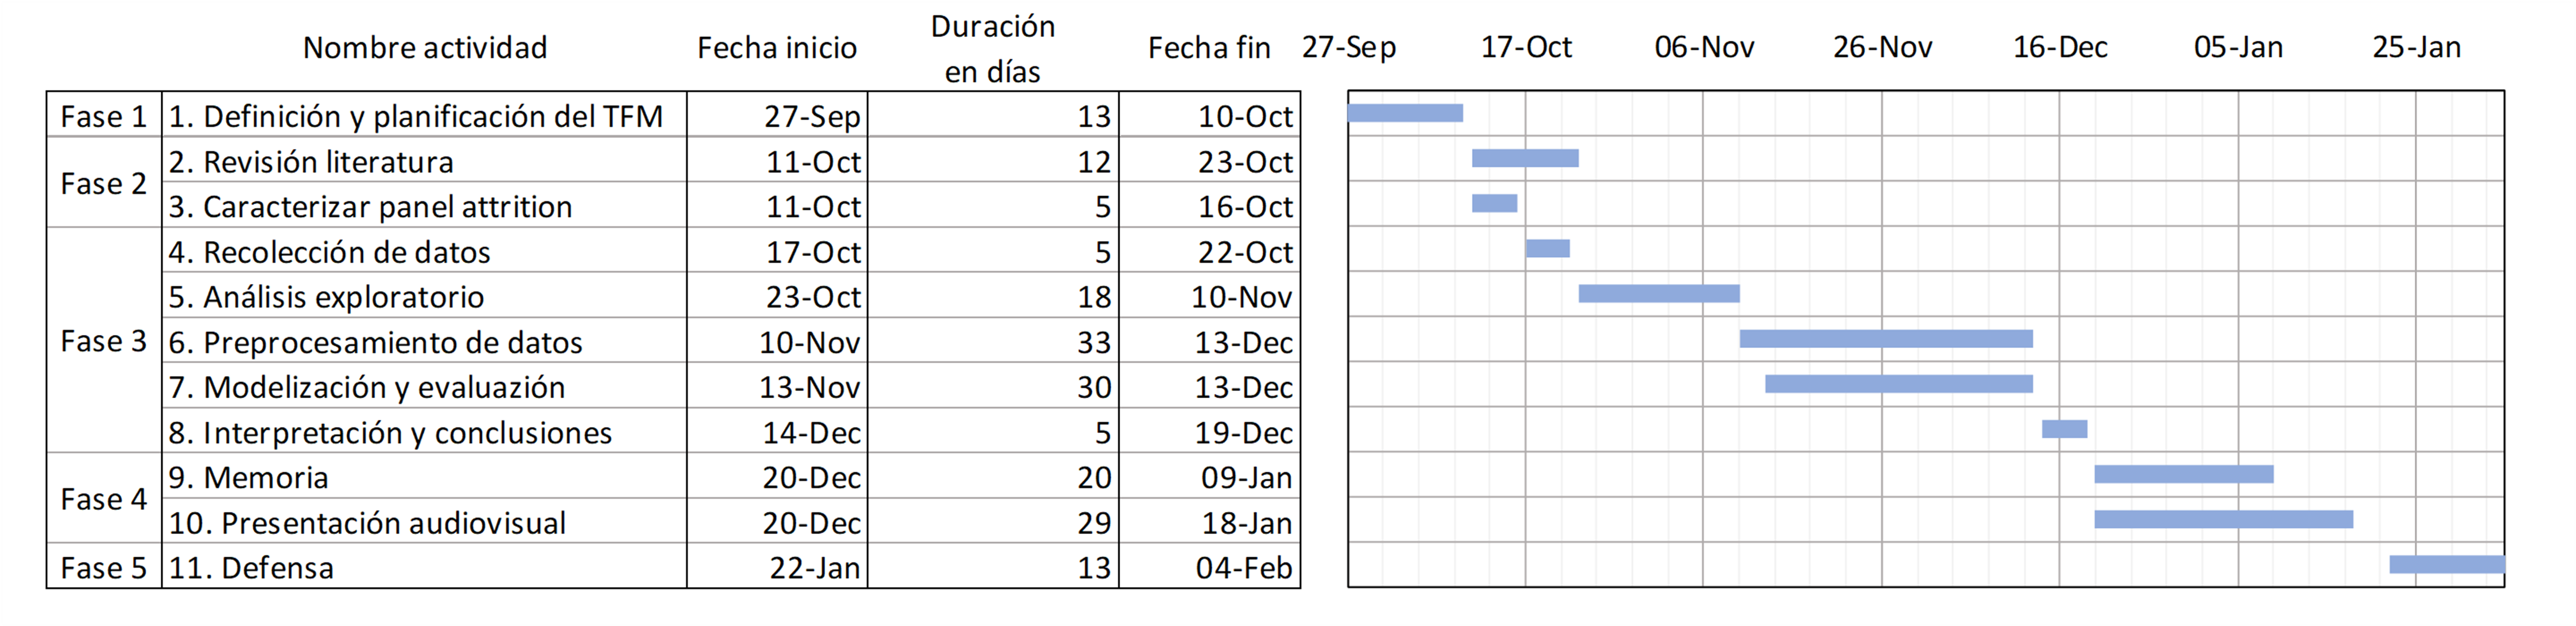
\includegraphics[width=1\textwidth]{figs/Gantt_diagram.png}
	\caption{Planificación de las actividades del TFM}
	\label{fig:gantt}
\end{figure}

\section{Motivación personal}

Trabajo para el Banco de España, y formo parte del equipo que elabora la Encuesta Financiera de las Familias (EFF) desde principios de 2015. He participado en la elaboración de sus cuatro últimas ediciones (EFF2014, EFF2017, EFF2020 y EFF2022) y con los años ha crecido mi interés por la metodología de encuestas y el potencial que tienen para recoger información sobre fenónemos que de otra manera serían difíciles de captar. La EFF es una fuente de información de referencia en el campo de las finanzas de los hogares y eso hace más importante realizar trabajos y esfuerzos para garantizar e incluso mejorar la calidad de sus datos. En ese sentido, la gran cantidad de paradatos que se generan durante cada ola ofrecen muchas oportunidades para aprender sobre todo el proceso y encontrar maneras de mejorarlo.

Por otro lado, en los últimos años ha aumentado cantidad de datos que se generan durante la encuesta y también su variedad, tomando espacecial relevancia los audios de las entrevistas y los comentarios de texto escritos por los entrevistadores, que se han convertido en herramientas fundamentales de los procesos de revisión de calidad de los datos. Los métodos y las herramientas desarrolladas en el campo de la ciencia de datos abren un mundo de posibilidades para poder analizar y explotar toda esa información.

Finalmente, sobre el Panel Attrition, considero que la etapa más importante de la elaboración de la EFF es el trabajo de campo. En ella se contacta a los hogares, se les convence para participar en la encuesta y se realizan las entrevistas. Marca el devenir las siguientes etapas, y también el nivel de calidad de los datos. Por esa razón, es importante conseguir la colaboración de los hogares. Especialmente la de los hogares panel, ya que representan una proporción importante de la muestra, y no convercerles puede llegar a ser muy costoso. Y es un área que en la EFF no se ha podido explorar hasta. Es una gran oportunidad para aprender.
\chapter{Panel attrition: causas, presencia en la EFF y predicción}
\label{chapter:attrition}
\section{Causas del panel attrition y cómo reducir su impacto durante la recolección de datos}

Conceptualmente, las causas del panel attrition pueden clasificarse en tres categorías condicionales (\cite{lepkowski2002nonresponse}): no-localización, no-contacto y no-cooperación.

La no-localización se refiere a no localizar exitosamente a un encuestado durante una ola posterior. Generalmente, esto se debe a cambios en la información de contacto (dirección de residencia, número teléfono, correo electrónico...) obtenida del participante durante la ola anterior (\cite{couper2009keeping}). Algunos factores que pueden contribuir al éxito o fracaso en la localización son el método de recolección de datos, la propensión a los cambios de localización de los encuestados entre diferentes olas, el tiempo transcurrido entre olas e incluso el presupuesto (\cite{lynn2009methods}). Por ejemplo, las encuestas con entrevistas cara a cara utilizan métodos de rastreo y búsqueda que suelen ofrecer altos índices de localización y cooperación (\cite{de2005mix}, \cite{couper2009keeping}), pero también requieren esfuerzos adicionales para localizar a los participantes panel que se hayan mudado, como por ejemplo reembolsar a los entrevistadores los gastos derivados del proceso de búsqueda.

Posteriormente, tras localizar al encuestado, es necesario establecer un contacto. En este paso el método de recolección de datos vuelve a ser muy importante. Por ejemplo, en una encuesta por correo postal o por email, el contacto depende de que el encuestado reciba dicho correo y además le preste atención. En cambio, en entrevistas presenciales en el hogar o entrevistas telefónicas, debe darse una coincidencia temporal entre la disponibilidad del entrevistado (está en casa o tiene su teléfono disponible) y el intento de contacto del entrevistador (realiza una visita su casa o llama por teléfono). En este sentido, dos estrategias de contacto que han presentado buenos resultados han sido utilizar un número de intentos de contacto alto y diversificado en horarios (mañana, tarde, fines de semana...), y establecer períodos para realizar entrevistas lo suficientemente largos (\cite{nicoletti2005survey}, \cite{watson2009identifying}). Además, las encuestas longitudinales ofrecen la ventaja de poder utilizar datos sobre el proceso de recolección en olas anteriores, y diseñar mejores estrategias de contacto o identificar casos en los que el contacto puede ser complicado (\cite{calderwood2012using}, \cite{lagorio2016call}).

Finalmente, cuando se ha establecido contacto con el encuestado. éste puede cooperar de nuevo con los encuestadores, o por el contrario rechazar hacerlo. La falta de cooperación es una preocupación común en las encuestas, y hay bastante literatura sobre las motivaciones que puede haber detrás de los rechazos. Suelen destacar factores relacionados con las características de los participantes, como características sociodemográficas (edad, sexo, nivel de salud...) o el entorno (composición del hogar, del barrio de resdiencia...); con el diseño de la encuesta, como la temática de las preguntas o el método de recolección de datos; y con las características de los entrevistadores, como su apariencia o la experiencia previa realizando encuestas (\cite{groves1992understanding},\cite{obrien2006sensitive}. En el caso de las encuestas longitudinales, los encuestados ya tienen una experiencia previa sobre la encuesta que puede hacer potenciar el efecto de factores como la duración de la entrevista, la carga cognitiva que supone pensar las respuestas, la sensibilidad sobre la temática o la fatiga por haber participado ya en varias ediciones (\cite{laurie1999strategies}, \cite{watson2009identifying}, \cite{lynn2018tackling}). Pero, al igual que con los contactos, las encuestas longitudinales también poseen información sobre el proceso de contacto, el desarrollo de la entrevista y las características de los encuestados en olas anteriores que pueden ayudar a diseñar incentivos que contribuyan a la cooperación (\cite{laurie2009use}) o descubrir la influencia de los entrevistadores para convencer a los encuestados, y lo importante que es su continuidad entre olas (\cite{lynn2014continuity}).

\section{Falta de respuesta y panel attrition en la Encuesta Financiera de las Familias}

La Encuesta Financiera de las Familias es una encuesta longitudinal en la que se entrevista a hogares residentes en España. Su primera edición se realizó en el año 2002, y se ha producido de manera trienal hasta el año 2020. Desde entonces, su producción es bienal, siendo la ola de 2020 la primera planificada para ser publicada con esta nueva frecuencia.

El objetivo de su primera edición era captar bien la distribución de la riqueza de los hogares españoles, por lo que el diseño de su muestra se fundamentó en un sobremuestreo de hogares con mayor nivel de riqueza\footnote{El diseño del sobremuestreo de la EFF toma como referencia la \href{https://www.federalreserve.gov/econres/scfindex.htm}{Survey of Consumer Finances (SCF)}, que es la encuesta equivalente a la EFF en Estados Unidos, y que elabora la Reserva Federal. Lo ejecuta el Instituto Nacional de Estadística, con la colaboración de la Agencia Tributaria. El nivel de riqueza de los hogares se obtiene a partir de la declaraciones individuales más recientes en el impuesto sobre el patrimonio que hay en España (facilitado por la Agencia tributaria), y se definen unos estratos de riqueza a partir de los intervalos de la SCF y los percentiles de la distribución del nivel de riqueza de los hogares. Los hogares en los estratos más altos tienen mayor probabilidad de ser seleccionados. Para las regiones de País Vasco y Navarra no se realiza sobremuestreo porque no se dispone de información} (\cite{effmethod2002}). Desde la siguiente edición (EFF2005) en adelante, además de mantener la representatividad de la muestra para el año de la ola correspondiente, se incluyó como objetivo adicional el incluir un componente longitudinal que consistía en volver a preguntar a todos los hogares que participaron en la ola anterior, y así poder hacer análisis de causalidad. Para conseguir ambos objetivos, en las ediciones de 2005, 2008 y 2011 se implementaron muestras de refresco por estrato de riqueza para complementar a la muestra panel que venía de olas anteriores (\cite{effmethod2005}, \cite{effmethod2008},  \cite{effmethod2011}). Finalmente, en la edición de la EFF2014 se estableció el límite máximo de participación de los hogares en cuatro olas consecutivas, y desde entonces se eliminan de la muestra longitudinal a aquellos hogares que ya han participado en cuatro olas consecutivas (\cite{effmethod2014}, \cite{effmethod2017}).

El proceso de recopilación de los datos se basa en la realización de entrevistas personales, generalmente en la residencia de los hogares seleccionados. Los entrevistadores deben localizar la vivienda en la que reside del hogar, realizar varias visitas en diferentes combinaciones de horarios y días de la semana\footnote{De manera general, unos días antes de la primera visita, la empresa de campo envía una carta al hogar, firmada por el gobernador del Banco de España, para informarle de que ha sido seleccionado para participar en la EFF, y que en los próximos días recibirá la visita de una persona para concertar una cita para una entrevista personal. A algunos hogares panel también se les contacta por teléfono si mostraron alguna preferencia por ser contactados de esa manera.}, pedir su colaboración con la EFF y concertar una cita para realizar la entrevista\footnote{Los hogares que aceptan participar y completan la entrevista reciben un obsequio por parte del Banco de España. Los hogares panel también reciben otro obsequio por haber participado en la edición anterior, independientemente de que accedan a participar de nuevo.}. Este procedimiento es el mismo tanto para la muestra de refresco como para la muestra panel. La participación es completamente voluntaria, la información es confidencial, y los hogares pueden decidir interrumpir la entrevista o pararla en cualquier momento.

El Banco de España incluye un análisis de la falta de respuesta y de panel attrition en los documentos metodológicos de cada ola de la EFF (\cite{effmethod2002}, \cite{effmethod2005}, \cite{effmethod2008}, \cite{effmethod2011}, \cite{effmethod2014}, \cite{effmethod2017}). En estos análisis se muestran, diferenciando entre muestra panel y muestra no panel, el número de hogares contactados por tipo de respuesta (completas, rechazos, no contactados...), las tasas de cooperación según el estrato de riqueza de los hogares contactados, y los odd-ratios de dos modelo logit de cooperación frente a rechazo en el que se utilizan diferentes categorías recogidas por los entrevistadores sobre las condiciones de los edificios, del nivel socioeconómico del barrio, el tamaño del municipio de residencia en número de habitantes y la región de residencia. En general se observa que se contacta con más hogares no panel que con hogares panel, pero es un resultado esperable porque sus tasas de cooperación también son más bajas que las de la muestra panel. Esto se mantiene tanto para la totalidad de la muestra como diferenciando por estrato de riqueza. También se observa que para ambos tipos de muestra las tasas de cooperación tienden a ser menores a medida que aumenta el estrato de riqueza de los hogares. Con respecto a los modelos logit, los resultados difieren entre entre olas ya que en una ola son estimadores son significativos, pero en otra no lo son. Aún así, algunas tendencias sí se han observado de manera repetida en la mayoría de olas son que la probabilidad de cooperar decrece cuando aumenta el tamaño del municipio\footnote{Este efecto siempre es negativo para la muestra no panel en todas las olas, pero para la muestra panel hay algunas olas para las que su efecto no es significativo.}, que la probabilidad de no cooperar aumenta para barrios con menor nivel económico, y que existen diferencias en la cooperación entre regiones. Sin embargo, es posible que el efecto regional esté afectado por algún tipo de efecto de entrevistador, ya que los entrevistadores suelen hacer sus entrevistas en las mismas regiones ola tras ola.

Estos análisis que acabamos de describir muestran que existe no respuesta y panel attrition en la EFF. Pero se limitan a hacer una comparación de cada edición con la inmediatamente anterior. No se observa cuántos hogares suelen completar las cuatro olas para las que han sido seleccionadas, ni la distribución de los abandonos con el paso de las olas. Por otro lado, a la hora de analizar la no respuesta de muestra panel no se utiliza información recogida durante la ola anterior que podría ser relevante para analizar el panel attrition, como por ejemplo las características de los hogares, el número de intentos de contacto en la edición anterior, o la duración de la entrevista de la ola anterior.

La EFF ofrece muchas oportunidades para poder investigar sobre la falta de respuesta y el panel attrition en esta encuesta, ya que hay muchos análisis que no se han podido realizar. Conocer las causas que pueden provocar el panel attrition en la EFF ayudará a desarrollar herramientas que ayuden a combatirlo, y con ello mejorar las tasas de respuesta de los hogares y la calidad de los resultados de la encuesta.

\section{Predicción de Panel Attrition}

La regla tradicional utilizada para diseñar encuestas ha sido la estandarización de todos los procesos y protocolos. Todas unidades muestrales deben ser tratadas de la misma manera. Con la excepción de las introducciones de los entrevistadores (\cite{groves1992understanding}), esta regla se mantuvo durante bastante tiempo. Pero el aumento de las reticencias de la población a participar en encuestas y los recortes presupuestarios llevó a buscar cómo mejorar la eficiencia de los procesos de elaboración de encuestas, y empezaron a considerarse diseños adaptativos enfocados a subgrupos específicos de la muestra (\cite{groves2006responsive}, \cite{lynn2014targeted}, \cite{lynn2017standardised}). En ese sentido, la predicción se ha convertido en una opción muy interesante para poder identificar anticipadamente a individuos que potencialmente podrían abandonar precipitadamente una encuesta longitudinal, y en los que los métodos de machine learning tienen un peso importante ya que no necesitan un conocimiento previo de las relaciones que se quieren estudiar, y suelen adaptarse bien a contextos en los que la relación entre la variable dependiente y sus predictores suele ser compleja y no lineal (\cite{buskirk2018introduction}, \cite{kern2019tree}, \cite{kern2021predicting}, \cite{jankowsky2022validation}).

Los estudios de modelos predictivos realizan una comparación de rendimiento entre modelos tradicionales utilizados para analizar panel attrition, casi siempre una regresión logística, y modelos basados en métodos de Machine Learning, como diferentes tipos de árboles de decisión o máquinas de soporte de vectores. \cite{kern2019tree} y \cite{kern2021predicting} muestran casos en los que los modelos predictivos basados en machine learning, especialmente árboles de decisión, presentan resultados prometedores. Sin embargo, en \cite{jankowsky2022validation} apenas observan diferencias significativas entre los resultados de un modelo de regresión logística y los de un modelo GBM (Gradient Boosting Machine). La conclusión de ese artículo es que no necesariamente un modelo más complejo (y más complejo de entender) puede ser más adecuado para predecir panel attrition, y por tanto utilizarse para diseñar políticas adaptativas para reducirlo.

La intención de este proyecto es realizar un estudio similar a los propuestos por \cite{kern2021predicting} y \cite{jankowsky2022validation}, y comprobar si modelos basados en métodos de machine learning pueden predecir adecuadamente el panel attrition en la EFF, y dar la posibilidad de contribuir al desarrollo de herramientas que ayuden a reducirlo.
\chapter{Datos y metodología}
\label{chapter:datos_metodologia}

\section{Datos: La Encuesta Financiera de las Familias}\label{section:datos}

Para este proyexto se van a utilizar los datos de la Encuesta Financiera de las Familias (EFF). La EFF es una encuesta oficial a hogares elaborada por el Banco de España y está incluida en el Plan Estadístico Nacional. Su primera edicion se realizó en el año 2002, y se ha producido de manera trienal hasta el año 2020. Desde entonces, se produce de manera bienal.

El objetivo de la EFF es recabar información sobre las condiciones financieras de los hogares residentes en España. Su cuestionario principal está compuesto por nueve secciones. Las secciones 1 y 6 recogen información sociodemográfica individualizada de todos los miembros del hogar y también información individualizada sobre la situación laboral y los ingresos de cada miembro del hogar mayor de 16 años. El resto de secciones recogen información detallada sobre los activos, deudas, gastos y uso de medios de pago del hogar en su conjunto, y contienen módulos específicos que recogen información individualizada de ciertos elementos patrimoniales si el hogar los posee, como propiedades inmobiliarias, negocios gestionados por cuenta propia o planes de pensiones. Los hogares formados por más miembros mayores de edad y que posean más elementos patrimoniales responderán a más preguntas. Por poner un ejemplo con números, en la EFF2017 a cada hogar se le plantearon entre 137 y 594 preguntas, siendo la mediana de 259 preguntas (\cite{effmethod2017}).

La EFF es la única fuente estadística que permite relacionar información sobre activos, deudas, ingresos y gastos de los hogares españoles. Esto permite analizar las decisiones de inversión y financiación de las familias y conocer su situación patrimonial, y gracias a ello tener un mayor conocimiento de la economía española y poder utilizarlo para hacer un diseño adecuado de politicas públicas. Por nombrar algunos ejemplos de estudios realizados con la EFF, se ha utilizado para cuantificar el ahorro adicional generado para los partícipes en planes de pensiones de empresa (\cite{gomez2022pensiones}), para caracterizar cómo afectó la pandemia del Covid-19 a la situación patrimonial de los trabajadores más afectados por dicha crisis (\cite{alvargonzalez2020pandemia} o para analizar las diferencias en aceptación y uso de tarjetas de crédito y banca online entre diferentes grupos de hogares desde el año 2002 (\cite{crespo2023bancaonline}).

El diseño de la muestra de la EFF tiene dos características importantes: un sobremuestreo de hogares ricos y un componente longitudinal o panel. El sobremuestreo de ricos\footnote{La muestra de la EFF es seleccionada por el Instituto Nacional de Estadística, en colaboración con la Agencia Tributaria, a partir de las declaraciones individuales más recientes en el Impuesto sobre el Patrimonio. Para una descripción más detallada del proceso, puede consultarse \cite{effmethod2017}.} garantiza poder analizar con suficiente precisión el comportamiento de los hogares de la parte alta de la distribución de riqueza. Este detalle es importante porque la distribución de la riqueza entre los hogares es asimétrica, por lo que sólo unos pocos hogares, especialmente los más ricos, son los que invierten en ciertos activos. Por otro lado, el compomente panel indica que se vuelve a entrevistar a hogares que participaron en ediciones anteriores. Esto permite monitorearles durante períodos de hasta diez años, y observar los cambios en las variables de interés de la encuesta. El número máximo de ediciones en las que un hogar puede participar en la EFF es de cuatro olas consecutivas. Si cesa su participación antes de completar sus cuatro ediciones, se descarta de la muestra y no vuelve a ser contactado en olas posteriores. Finalmente, para sustituir a los hogares descartados del panel rotatorio y mantener la representatividad de la muestra, en cada nueva ola de la EFF se añade una nueva muestra de refresco a la muestra panel.

Volviendo a los datos, en este proyecto se utiliza información que proviene tanto de las respuestas al cuestionario de la EFF, como del paradata recopilado durante la producción de los datos. En la figura 4.1. puede observarse un resumen de este proceso. La producción de la EFF se divide en dos grandes fases: Campo y Post-Campo. Durante el Campo se contacta con los hogares, se realizan las entrevistas personales, se procesan los datos y se realiza parte de la revisión de los mismos. En el Post-Campo se termina el proceso de revisión, se evalúa el grado de no-respuesta de los datos de cada hogar para eliminar las entrevistas con poco contenido informativo, y se procede a la imputación de la no-respuesta. Tras este último proceso, se obtienen los datos finales.

\begin{figure}[h]
	\centering
	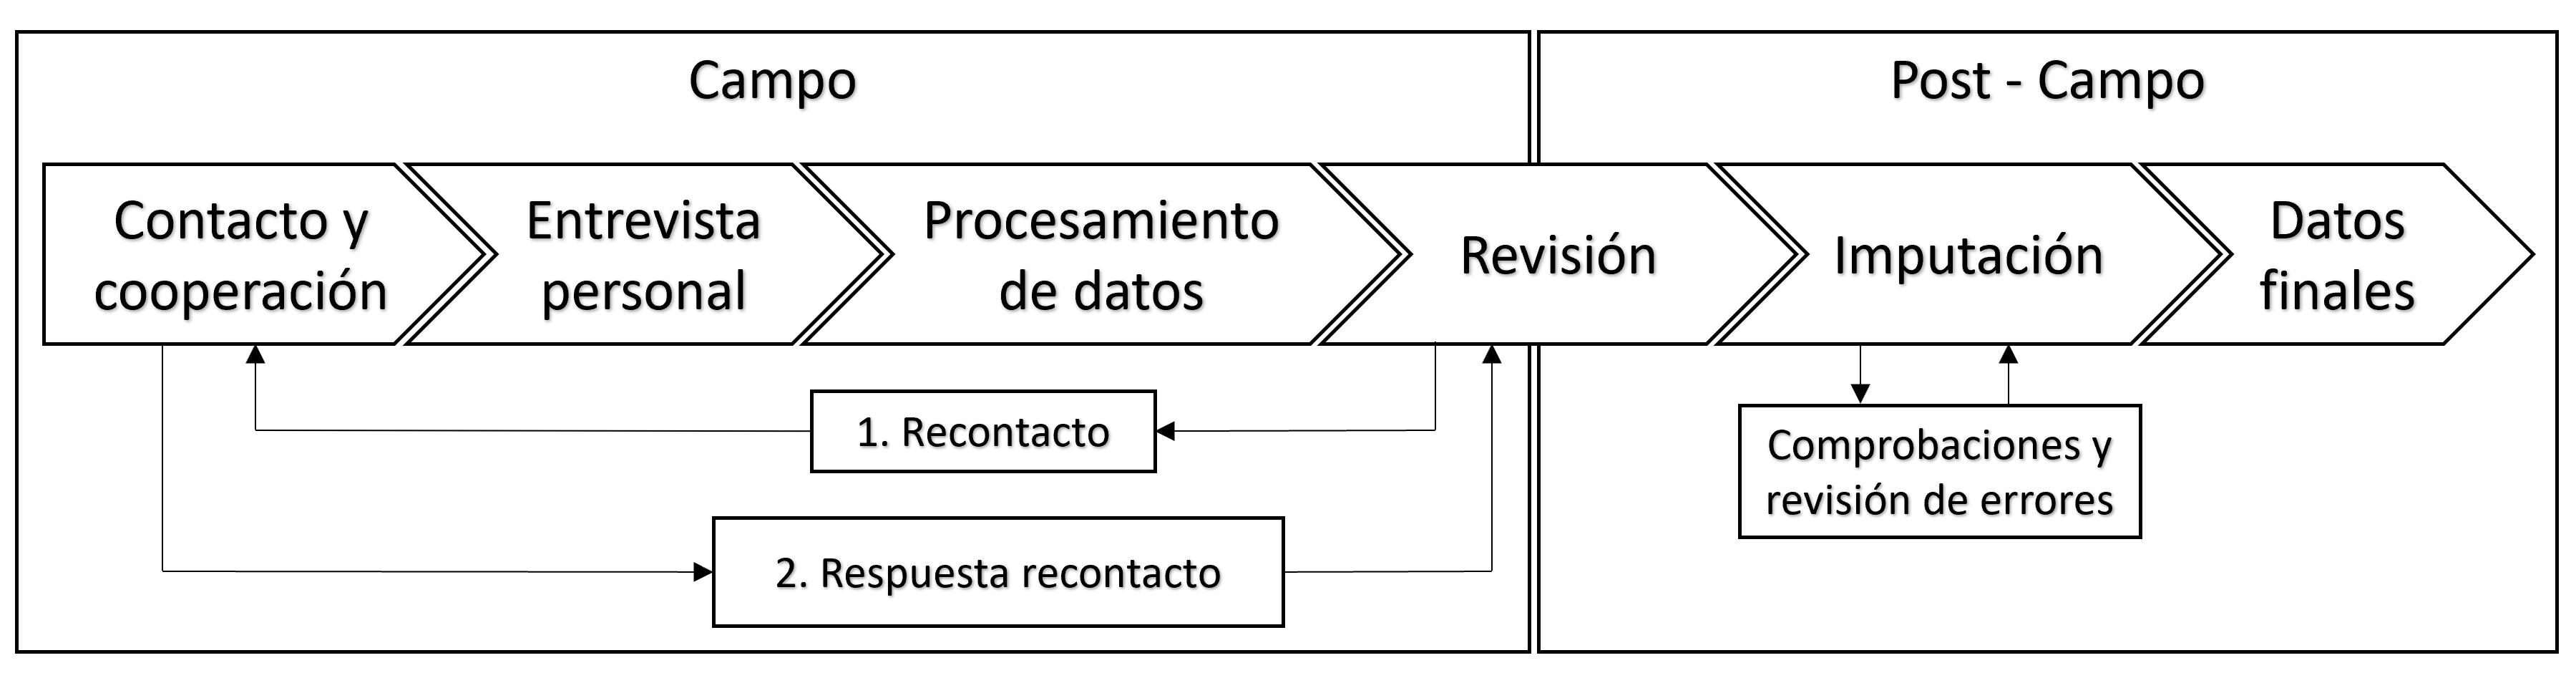
\includegraphics[width=1\textwidth]{figs/fases_creacion_datos_eff.png}
	\caption{Fases de la creación de datos de la EFF}
	\label{fig:eff_phases}
\end{figure}

A continuación se hace una breve descripción de los aspectos más relevantes de las subfases y que son importantes para la selección de variables para este estudio.

\begin{itemize}
    \item \textbf{Contacto y cooperación:} Los entrevistadores realizan visitas personales a los hogares en sus domicilios. Esto puede requerir varios intentos, ya que es necesario que algún miembro del hogar esté físicamente en su hogar cuando tenga lugar la visita presencial. La información sobre cada intento (fecha y hora, resultado...) se recoge en un ordenador. Antes de establecer el contacto, los entrevistadores rellenan un cuestionario que recoge información sobre las características del barrio y del edificio en el que vive el hogar.
    \item \textbf{Entrevista personal:} Se realiza una entrevista personal a la persona con más conocimiento de las finanzas del hogar, que se denomina Persona de Referencia o PR. La PR puede ser miembro del hogar, o un representante del mismo, demoninado proxy, siempre y cuando sea la persona con mayor conocimiento de las finanzas del hogar. También pueden participar otros miembros del hogar. Antes de empezar la entrevista, se pide a la PR su consentimiento para que algunas partes de la misma puedan ser grabadas en audio por motivos de calidad de los datos. La entrevista puede realizarse aunque no haya grabación. Los entrevistadores recogen las respuestas en un ordenador o una tablet (CAPI), y también pueden anotar en comentarios de texto todos los detalles que consideren importantes para la revisión. La PR puede decidir no contestar a ciertas preguntas. Su valor se asignará como missing, y se imputará más adelante. Las cantidades monetarias pueden responderse en valor puntual, o dentro de un rango de valores. Tras la entrevista, y sin la presencia de los hogares, los entrevistadores rellenan un cuestionario con información sobre el desarrollo de la entrevista, en el que por ejemplo se recoge el nivel de comprensión de la PR a las preguntas, el nivel de interés mostrado por la PR o cuántas personas han participado en la entrevista.
    \item \textbf{Procesamiento de datos:} Los ordenadores y servidores de la empresa de campo procesan los datos recogidos durante el contacto con los hogares y durante las entrevistas. Se crean tres ficheros, uno con las respuestas al cuestionario, uno con la información de los contactos con cada hogar, y finalmente uno con la información del paradata recogido por el ordenador durante la entrevista\footnote{También se crea un fichero con los comentarios de texto recogidos por los entrevistadores durante la entrevista, pero no se ha podido incluir en este estudio por falta de tiempo.}.
    \item \textbf{Revisión:} Un equipo de personas revisa individualmente todas las entrevistas y corrige los errores que puedan detectarse. Si hay información relevante que se ha recogido erróneamente o se ha omitido, se contacta de nuevo con el hogar para corregirlo o recuperar esa información. Este recontacto se hace por teléfono. Toda la información sobre la revisión (cambios sobre variables, recontactos...) se recoge en una aplicación informática y puede ser exportada en ficheros de diversos formatos (csv, excel...).
    \item \textbf{Imputación:} Se analiza la proporción de preguntas sin responder dentro de cada entrevista (no-respuesta), y se eliminan las que no superen ciertos umbrales de calidad. Todas las variables que contienen no-respuesta se imputan mediante técnicas de imputación múltiple\footnote{Los métodos de imputación múltiple utilizados en la EFF pueden consultarse en \cite{barcelo2006imputation}.}. Se crean 5 ficheros con datos imputados.
\end{itemize}

Con respecto a los procedimientos de Contacto y Entrevista personal, es necesario mencionar que algunos elementos tuvieron que modificarse durante la EFF2020, ya que el campo tuvo lugar entre noviembre de 2020 y junio de 2021, y se vió afectado por la pandemia del Covid-19. Durante esa ola, los entrevistadores siguieron visitando personalmente a los hogares para conseguir su colaboración\footnote{Durante el principio del campo, algunos hogares panel fueron contactados sólo por teléfono, pero a las pocas semanas se decidió establecer la visita personal como el procedimiento estándar.}, pero siempre respetando las medidas de distanciamiento social. Las entrevistas se realizaron de manera telefónica asistida por una tablet (CATI). El resto de procedimientos se mantuvieron como en otras ediciones.

Para la elaboración de este proyecto se utiliza la información recopilada durante las olas de la EFF2017, EFF2020 y EFF2022 \footnote{En el momento de escribir este documento, la EFF2022 se encontraba en pleno proceso de imputación, por lo que el equipo del Banco de España ya conocía los resultados de participación de esa ola y era posible utilizarlos para este proyecto.}. Estas ediciones son las únicas que cuentan con la información más detallada de paradata y de las características de los entrevistadores. En ediciones anteriores esta información o no está disponible, o contiene errores de medida que no son fácilmente corregibles. A pesar de esto, es posible identificar en cuántas ediciones ha participado cada hogar, por lo que es posible utilizar información que se remonta hasta la edición de la EFF2011. Los ficheros de datos que se han utilizado durante este proyecto son:

\begin{itemize}
    \item \textbf{Fichero de trabajo:} Registro de hogares con entrevistas válidas. Contiene la información de las respuestas de los hogares, incluyendo las correcciones y ediciones de la revisión. Se indican los datos que deben ser imputados. También incluye variables auxiliares generadas para el proceso de imputación (características del hogar, de los miembros, del municipio...) y contadores de no respuesta de cada entrevista. Es el fichero que se utiliza para imputar.
    \item \textbf{Fichero de datos imputados:} Registro de hogares que contiene las respuestas al cuestionario después de haber imputado los datos con no-respuesta de los hogares. Por simplicidad, sólo utilizaremos uno de los conjuntos de datos de la imputación multiple. Sólo contiene variables imputadas e indicadores de las características del hogar.
    \item \textbf{Fichero de contactos:} Registo de hogares contactados durante una ola de la EFF. Contiene información sobre el número de intentos de contacto con cada hogar, la fecha en que se produjo, el resultado de cada uno de ellos (aplazamientos, rechazos...) y las respuestas al cuestionario de vecindario rellenado por los entrevistadores.
    \item \textbf{Fichero de revisión:} Registro de hogares e incidencias que contiene información sobre el proceso de revisión y los recontactos. Para cada hogar hay varios registros. Uno contiene información general sobre el proceso de revisión (por ejemplo, si se ha realizado un recontacto), y el resto de registros son incidencias en los datos que se detectado (por ejemplo, si se ha omitido una propiedad inmobiliaria, se abrirá un registro indicando esa incidencia y cómo se ha solucionado).
    \item \textbf{Censo de entrevistadores:} Registro de entrevistadores que contiene la información disponible sobre los entrevistadores que han participado desde la EFF2014 a la EFF2022.
    \item \textbf{Fichero de paradata:} Registro con información sobre las pantallas del software CAPI que se utilizó durante la entrevista. Para cada hogar, contiene información detallada de la interacción del entrevistador con el ordenador durante la entrevista. En concreto, contiene el flujo de pantallas que se visualizaron en el ordenador en cada entrevista, y para cada pantalla se registra la fecha y hora en la que entró, si volvió a la pantalla anterior, o el tiempo que estuvo en cada pantalla.
\end{itemize}

\section{Metodología}

Tomando como referencia las estrategias de investigación propuestas en \cite{oates2022researching}, en este proyecto se presenta un 'Caso de estudio'. Se busca tener un conocimiento profundo sobre la participación de los hogares panel en el caso específico de la EFF, y buscar un modelo para predecirla.

La metodología de este proyecto se fundamenta en cuatro pilares. En primer lugar, en la recopilación de los datos de las entrevistas y los entrevistadores que participaron en las olas EFF2017, EFF2020 y EFF2022. El segundo pilar es la realización de un análisis descriptivo de un conjunto de variables con potencial para explicar la Attrition. En tercer lugar, en el entrenamiento de varios modelos basados en métodos de machine learning con datos de la EFF2017 y la EFF2020, y evaluar su rendimiento para predecir la participación de los hogares panel en la EFF2022. Para este ejercicio se adapta la implementación hecha en \cite{beste2023case} al caso de la EFF. Finalmente, se realiza una valoración de los resultados obtenidos y qué pasos podrían darse en el futuro para seguir desarrollando este proyecto.

El resto de esta sección se divide en tres apartados. Es primer lugar se da una breve descripción del proceso de recopilación de los datos. En el siguiente apartado se define la variable dependiente $Attrition$ y también las variables que se van a utilizar como predictores de los modelos. Finalmente, se cierra este capítulo con la descripción de la estrategia de entrenamiento y validación de los modelos.

\subsection*{Recopilación de datos}

Como acabamos de comprobar, en la EFF hay, por un lado, información sobre las entrevistas a los hogares repartida en varios ficheros para cada ola en la que han participado; y por otro lado, información sobre los entrevistadores que han colaborado en la EFF recogidas en un censo. La unidad de análisis de este estudio son hogares que ya han participado al menos una vez en alguna edición de la EFF, y que son elegibles para ser entrevistados en la siguiente edición. Por tanto, para cada ola se selecciona sólo a los hogares que han participado como máximo en tres ediciones, ya que los que han participado en la cuarta son eliminados de la muestra de cara a la siguiente edición. Los datos de una ola en concreto se utilizan como variables explicativas en los modelos, y como variable objetivo se extraerá el estatus de participación de ese mismo hogar del fichero de contactos de la ola siguiente. La vinculación de la información entre ambas ediciones se realiza a través de un identificador común que tienen los hogares en los ficheros de datos de ambas olas.

Por otro lado, la vinculación con la información del censo de entrevistadores se realiza a través de un identificador único que tiene cada entrevistador y que permanece inalterable a lo largo de las olas. Para cada hogar se conoce el identificador de la persona que realizó la entrevista en cada una de las olas en las que participó.

%\vspace{-5pt}

\subsection*{Variable Attrition y predictores}

El objetivo del estudio es encontrar un modelo para predecir si un hogar que ha participado en la ola $t$ de la EFF no volverá a participar en la siguiente ola $t+1$. Para ello, se define la variable \textit{Attrition} como una variable dicotómica que toma valor 0 si el hogar vuelve a participar, y valor 1 si no vuelve a participar:

\begin{equation}
Attrition =
  \begin{cases}
    0       & \quad \text{el hogar participa en la ola $t+1$} \\
    1  & \quad \text{el hogar no participa en la ola $t+1$}
  \end{cases}
\end{equation}

En el cuadro \ref{table:attrition} puede observarse que, en las olas de 2020 y 2022, la mayoría de los hogares panel volvieron a participar. Aunque parezca que sólo un ligero desbalance entre las observaciones de cada clase de Attrition, durante los primeros entrenamientos y evaluaciones de los modelos se comprobó que las predicciones se asignaban masivamente a la clase mayoritaria ($Attrition=0$). Para evitar esto, y dado el tamaño limitado de la muestra, previo al entrenamiento se procede al balanceo de la clase Attrition realizando un sobre-muestreo de dicha clase usando el algoritmo SMOTE (Syntetic Monirity Over-sampling Technique, \cite{chawla2002smote}).

\begin{table}[ht]
\centering{}
\begin{tabular}{lcc}
\textbf{Attrition}           & \textbf{EFF2020} & \textbf{EFF2022} \\ \hline
Participa (attrition = 0)    & 3830             & 3974             \\
No participa (attrition = 1) & 2107             & 1531             \\ \hline
\end{tabular}
\caption{\textit{Distribución de Attrition en EFF2020 y EFF2022}}
\label{table:attrition}
\end{table}

En el otro lado de un modelo de predicción se encuentran las variables que se eligen como predictores. Por definición, estas variables deben contener información conocida y observable antes de que se producza el fenómeno que se quiere predecir. En ese sentido, para predecir \textit{Attrition} en $t+1$ se utilizan como predictores variables que se corresponden con la ola anterior, la ola $t$. La selección de estas variables se ha inspirado en la realizada por \cite{beste2023case} y \cite{kern2021predicting}, y adicionalmente se han incluido otras variables de interés para la EFF, como por ejemplo si un hogar se ha recontactado durante la revisión o si la entrevista se realizó con un proxy. La selección final de 57 variables explicativas utilizadas en este estudio puede consultarse en el cuadro \ref{table:vars}.

\begin{table}[ht]
    \centering
    \begin{tabular}{|l|p{10cm}|}
    \hline
        \textbf{Fuente de información} & \textbf{Variables} \\ \hline
        Características del hogar & Número de adultos con empleo, Número de adultos jubilados, Propietario vivienda principal, Tamaño del hogar, Tiene otras propiedades, Tiene joyas, Posee negocios, Posee cuentas para pagos, Posee acciones que cotizan, Posee acciones que no cotizan, Posee renta fija, Posee fondos de inversión, Posee cuentas para no pagos, Posee planes de pensiones, Les deben dinero, Poseen vehículos, Percentil de renta, Percentil de riqueza Bruta, Pareja vive en el hogar, Poseen otros activos financieros, Tienen deuda, Tienen ingresos de activos, Hijos viven en el hogar, Nivel de satisfacción con la vida \\ \hline
        Características PR & Nivel de satisfacción con la vida, Es panel, Nivel educativo, Estado de salud, Edad, Estado Civil - Casada, Estado Civil - Viuda, Sexo, Situación laboral - Asalariado, Situación laboral - Jubilado, Situación laboral - Inactivo \\ \hline
        Valoraciones FI & Recelo tras la entrevista, Edificio Unifamiliar, Barreras - portero automático, Barreras - Sin barreras, Entendimiento de las preguntas por parte de PR, Interés de PR, Razones colaborar - Interesado en estos estudios, Razones para colaborar - Lo lleva el BdE, Razones para colaborar - Relevancia de la encuesta, Razones - Favor al entrevistador, Razones - Dar su opinión, Razones - Otras \\ \hline
        Paradata & PR consiente grabar la entrevista, Hogar recontactado, Número de olas en las que se ha participado, Tamaño del municipio, Entrevista con proxy, Número de miembros del hogar que participan en la entrevista, Porcentaje de preguntas monetarias respondidas en valor puntual, Porcentaje de preguntas monetarias respondidas (incluye intervalos), Número de variables con valores missing, Duración de la entrevista en segundos \\ \hline
    \end{tabular}
    \caption{Selección de variables para entrenar los modelos de predicción}
    \label{table:vars}
\end{table}

\subsection*{Entrenamiento, validación y test de modelos de machine learning}

La estrategia de entrenamiento y validación utilizada en este proyecto se inspira en la implementada en \cite{beste2023case}. Se entrenan cuatro modelos de predicción basados en algoritmos de machine learning, y se compara su rendimiento con un modelo de referencia que se utiliza tradicionalmente para analizar Panel Attrition. Este modelo base es una Regresión Logística o Logit de efectos primarios (sin interacciones entre variables y sin especificaciones no lineales). Los modelos de machine learning que se entrenan y evalúan son un árbol de decisión (CART), un Random Forest (RF), un eXtreme Gradient Boosting (XGBOOST) y un Naive Bayes (NB). La elección de estos modelos se fundamenta, por un lado, en los buenos resultados que han mostrado para predecir panel attrition en otras encuestas para hogares (\cite{kern2019tree}, \cite{kern2021predicting}, \cite{beste2023case}) y, por otro lado, en que estos modelos son fácilmente interpretables en comparación con otros algoritmos de machine learning, como pueden ser las máquinas de soporte venctorial(SVM) o las redes neuronales. Esto facilita que sean utilizados para diseños adaptativos y reactivos.

Con respecto al proceso de entrenamiento y evaluación, a la hora de elegir los conjuntos de entrenamiento, validación y test, se tiene en cuenta el uso que se querría dar al algoritmo en la práctica. El objetivo es predecir qué hogares tienen más probabilidad de abandonar el estudio en la ola siguiente antes de que ésta tenga lugar. Por un lado,Eso implica establecer un criterio de separación temporal entre los conjuntos de entrenamiento y test, y asegurar que en los predictores de los modelos sólo se incluye información conocida ex-ante. En ese sentido, siguiendo la idea propuesta en \cite{beste2023case}, utilizaremos exclusivamente información disponible en una ola concreta para predecir el resultado de la participación en la siguiente. Por esa razón, para el entrenamiento y la validación de los modelos, se utiliza la información recopilada en la EFF2017 para predecir la participación en EFF2020, y para el ejercicio del test se utiliza la información recopilada en la EFF2020 para predecir la participación en la EFF2022.

Para el tuning de los hiperparámetros de los modelos, se sigue una estrategia de k-fold cross-validation para los conjuntos de entrenamiento y validación, con k=5. Con respecto a los valores específicos de los hiperparámetros, como no existe certeza sobre cuáles son los valores más adecuados, se considera un rango bastante amplio para cada hiperparámetro de todos los algoritmos. Para los modelos Logit y CART se utiliza un algoritmo de búsqueda de red (grid search) para probar cada combinación de hiperparámetros. Con respecto a los algoritmos RF y XGBOOST, dados los elevados tiempos y costes de ejecución de cada uno, se utiliza un algoritmo de búsqueda aleatoria (random search) con 2500 iteraciones. Aunque no se prueben todos los valores de los hiperparámetros, se ha comprobado que la búsqueda aleatoria es una alternativa válida en contextos de alta dimensionalidad de hiperparámetros (\cite{bergstra2012random}). Finalmente, a la hora de seleccionar las mejores combinaciones de modelos, la métrica que se busca maximizar es la ROC AUC.
\chapter{Resultados}
\label{chapter:resultados}

\section{Análisis exploratorio de los datos}
\label{section:exploring}

El objetivo del análisis exploratorio de datos es investigar las características de los datos que se van a utilizar. Por un lado, se observan las características particulares de cada variable, y por otro las relaciones que existan entre ellas, y de manera especial la que tienen con la variable Attrition. Esta información es importante porque ayuda a identificar y tratar rasgos de las variables que pueden afectar a los modelos de machine learning que se quieren entrenar.

Como veremos a continuación, en este proyecto se ha manejado una gran cantidad de datos de gran diversidad de origen y formato. El análisis exploratorio de toda esa información es muy amplio y no es posible incluir todo el trabajo en esta sección. Por esa razón, sólo se muestran resultados que son de interés para el análisis del panel attrition, o resultados que han ayudado a la toma de decisiones para la selección o transformación de variables para los modelos de predicción. 

Este análisis se separa en cinco bloques. El primero describe la gran cantidad de datos que se generan en la EFF y el proceso de filtrado que se ha realizado para este proyecto. Los tres boques siguientes abordan tres temas que preocupan a los productores de encuestas porque suelen afectar a la participación de los panelistas: la experiencia en la encuesta y las entrevistas, la persona que responde a la encuesta, y las características de los hogares. Finalmente, se aborda el problema de valores atípicos detectados en las duraciones de las entrevistas.

\subsection*{Número de registros y variables}
\label{section:registers_variables}

Una sola edición de la EFF produce una gran cantidad de datos. El Cuadro \ref{table:registers} muestra el número de registros y variables disponibles en cada uno de los ficheros utilizados en este proyecto. Estos números incluyen a todos hogares contactados y a todas variables generadas durante la producción de datos de la EFF en sus ediciones de 2017, 2020 y 2022\footnote{De la EFF2022 sólo se utiliza el fichero de contactos ya que sólo se necesita la información sobre la participación de los hogares panel en dicha edición.}. Tras realizar el filtrado de hogares elegibles para el estudio, se obtiene que los hogares de la EFF2017 elegibles para la EFF2020 son 5,937\footnote{Originalmente se identificaron 5938 hogares de la EFF2017 elegibles para la EFF2020. Pero uno de esos hogares no tenía registros en el fichero de paradata, y se eliminó del conjunto de datos final.} y los hogares elegibles de la EFF2020 para la EFF2022 son 5,505. Con respecto al censo de entrevistadores, sus números incluyen a los 260 entrevistadores que han participado en las ediciones de 2014, 2017, 2020 y 2022. Tras filtrar por las ediciones de 2017 y 2020, se obtiene que en la EFF2017 participaron 69 entrevistadores, mientras que en la EFF2020 participaron 65 entrevistadores, de los cuales 25 personas también participaron en la EFF2017.

\begin{table}[ht]
\centering{}
\begin{tabular}{lcccc}
\cline{2-5}
                            & \multicolumn{2}{c}{\textbf{EFF2017}}        & \multicolumn{2}{c}{\textbf{EFF2020}}        \\ \cline{2-5} 
\textbf{Nombre del fichero} & \textbf{Registros}   & \textbf{Variables}   & \textbf{Registros}   & \textbf{Variables}   \\ \hline
Fichero de trabajo          & 6,413                & 6,103                & 6,313                & 6,497                \\
Fichero de datos imputados  & 6,413                & 659                  & 6,313                & 787                  \\
Fichero de contactos        & 14,456               & 640                  & 15,457               & 636                  \\
Fichero de revisión      & 44,760               & 22                   & 35,217               & 51                   \\
Fichero paradata            & 2,807,091            & 13                   & 3,121,437            & 12                   \\ \hline
                            & \multicolumn{1}{l}{} & \multicolumn{1}{l}{} & \multicolumn{1}{l}{} & \multicolumn{1}{l}{} \\
                            & \multicolumn{4}{c}{\textbf{EFF2022}}                                                      \\ \cline{2-5} 
\textbf{}                   & \multicolumn{2}{c}{\textbf{Registros}}      & \multicolumn{2}{c}{\textbf{Variables}}      \\ \cline{2-5} 
Fichero de contactos        & \multicolumn{2}{c}{15,182}                  & \multicolumn{2}{c}{636}                     \\ \hline
                            & \multicolumn{1}{l}{} & \multicolumn{1}{l}{} & \multicolumn{1}{l}{} & \multicolumn{1}{l}{} \\
\multicolumn{5}{c}{\textbf{Censo de entrevistadores}}                                                                   \\ \hline
\multicolumn{2}{c}{\textbf{Registros}}             & \multicolumn{3}{c}{\textbf{Variables}}                             \\ \hline
\multicolumn{2}{c}{260}                            & \multicolumn{3}{c}{56}                                             \\ \hline
\end{tabular}
\caption{\textit{Número de registros y variables de los ficheros de datos}}
\label{table:registers}
\end{table}

En el cuadro \ref{table:registers} también puede observarse que hay ficheros que almacenan más de 6,000 variables. Esto supone un problema de dimensionalidad ya que hay más variables que registros en los datos. Sin embargo, hay cuatro maneras para reducir drásticamente el número de variables a manejar sin perder información relevante, y obtener las variables mencionadas en el cuadro \ref{table:vars}. La primera es que la inmensa mayoría de variables almacenan las respuestas al cuestionario principal de la EFF. En el segundo párrafo de la sección \ref{section:datos} se comentó que el número de preguntas que se formulan depende del número de miembros del hogar, sus edades, y los activos y deudas que posea el hogar, y que en la EFF2017 se plantearon entre 137 y 594 preguntas a cada hogar. Como los modelos de predicción requieren de variables que contengan datos para todos los registros, es posible descartar muchas variables por no tener valores para todos los hogares.

La segunda razón para descartar variables es que muchas no son informativas en su estado original y necesitan ser combinadas con otras para poder obtener información interpretable, o se utilizan como apoyo para la imputación. Por ejemplo, la información sobre cantidades monetarias se recoge en cuatro variables que permiten declarar valores en intervalos a los hogares que no quieran o no puedan dar un valor puntual (\cite{effmethod2017}). Esto se utiliza en la imputación para estimar valores puntuales dentro del rango declarado por el hogar. Al usar el fichero de datos imputados para entrenar los modelos, todas esas variables auxiliares se descartan.

En tercer lugar, hay variables duplicadas porque están almacenadas en varios ficheros de datos, por lo que sólo es necesario extraerlas de uno de esos ficheros. Por ejemplo, todas las variables que aparecen en el fichero de datos imputados también aparecen en el fichero de trabajo. Del fichero de trabajo se extraen indicadores de no-respuesta y otras variables de interés que no aparecen en el fichero de datos imputados, y de éste último se extraen las variables con los valores missing imputados.

Finalmente, para que los modelos de predicción puedan aplicarse tanto para datos de la EFF2017 como para la EFF2020, sólo se seleccionan las variables que estaban disponibles en ambas olas. Esta tarea ha requerido una gran dedicación de esfuerzo y tiempo, ya que en algunos ficheros se detectaron variables que no mantuvieron su nomeclatura, el tipo de dato almacenado o la codificación de los datos entre diferentes olas. Para asegurar la homogeneidad, se ha revisado de manera individualizada la nomenclatura y la codificación de cada variable para ambas ediciones de la EFF.

\subsection*{La experiencia en la encuesta y las entrevistas}

En la sección \ref{section:causes_attrition} se comentó que los hogares panel poseen experiencia previa sobre la encuesta que puede afectar a su participación en olas posteriores. Esta experiencia puede abarcar varias ediciones, pero también puede ser informativo observar datos sobre la ola más reciente.

En la figura \ref{fig:fig1} hay cuatro gráficos de mekko que muestran cómo fue la participación en la EFF2020 de hogares elegibles de la EFF2017 según su ola de entrada en la EFF, si consintieron grabar la entrevista de la EFF2017, si dicha entrevista se realizó con un proxy, y el nivel de recelo que mostraron después de realizarla. Los gráficos de mekko son gráficos de columnas apiladas 100\% en los que la anchura de cada columna muestra la proporción de hogares que hay de una categoría dentro de la muestra. Las regiones superiores o rojas de cada columna muestran la proporción de hogares que no participaron en la EFF2020, mientras que las regiones inferiores o azules muestran la proporción de hogares que sí participaron.

\begin{figure}[ht]
	\centering
	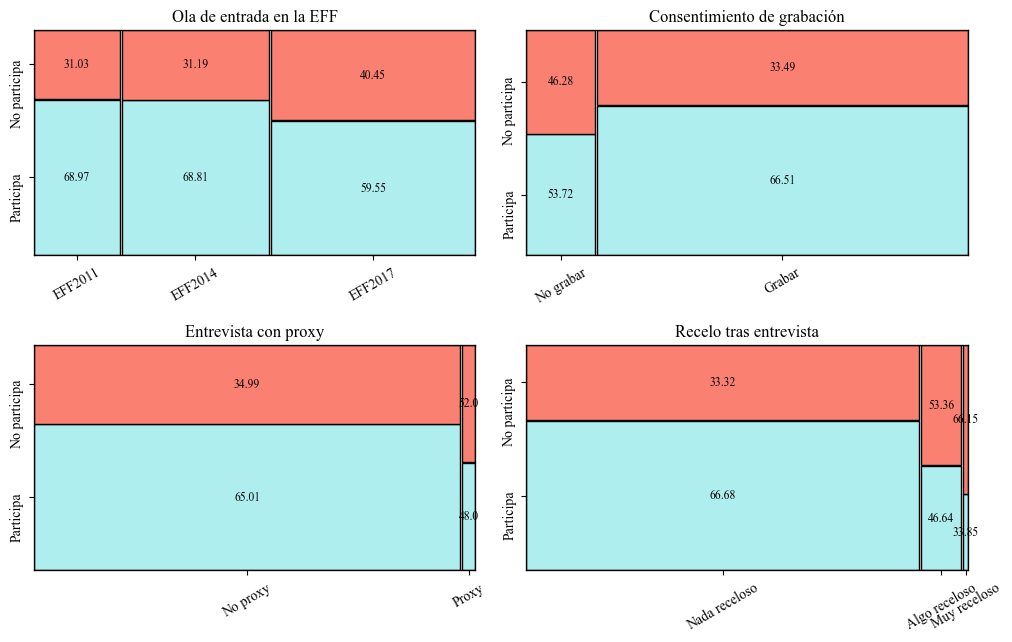
\includegraphics[width=1\textwidth]{figs/figure1.png}
	\caption{Participación en EFF2020 por experiencia en la EFF y en la entrevista de EFF2017}
	\label{fig:fig1}
\end{figure}

En la figura superior izquierda de la figura \ref{fig:fig1} se observa que la proporción de abandono de hogares que participaron por primera vez en 2017 es mayor que la de los que lo hicieron por primera vez en 2014 o en 2011, y entre estas dos últimas la proporción es similar. Esto sugiere que los hogares que van a participar en su segunda ola podrían ser más complicados de retener que los que llevan más tiempo. 

La figura superior derecha muestra que la proporción de no participación es mayor entre los hogares que no consintieron grabar la entrevista en 2017. Esto puede ser una señal de recelo hacia la encuesta, lo que puede dificultar la participación en las siguientes ediciones. En ese sentido también es interesante ver si los hogares se mostraban recelosos tras la entrevista, que es lo que se observa en la figura inferior derecha. La gran mayoría de hogares no se mostraron recelosos tras la entrevista, pero se observa que la proporción de hogares que no participaron en la EFF2020 es mayor a medida que aumenta el nivel de recelo.

Finalmente, en la figura inferior izquierda, se ve que la proporción de abandonos en 2020 fue mayor entre los hogares que hicieron la entrevista con proxy en 2017. Una situación que ha ocurrido bastantes veces en la EFF y que puede encajar con un abandono es el de un hogar formado por personas muy mayores en el que quien lleva las finanzas y termina respondiendo a la entrevista es un hijo o un familiar. Muchos de estos familiares se muestran muy recelosos y, comprensiblemente, quieren que no se moleste a sus familiares. En este tipo de situaciones puede ser más importante volver a convencer a estos familiares que a los propios miembros del hogar, ya que al final son ellos quienes conocen la información del hogar.

Algunos de estos resultados pueden parecer poco útiles porque es razonable pensar que un hogar que se mostró receloso durante la entrevista seguramente será más complicado de convencer para volver a participar en la siguiente edición. Sin embargo, para un entrevistador que está a punto de entrevistar a un hogar, puede ser muy útil saber si ese hogar se mostró receloso tras la anterior entrevista. A la hora convercer al hogar puede centrarse más en utilizar argumentos relacionados con la confidencialidad y la seguridad de los datos y no tanto en hablar de la relevancia de la encuesta o del eco que ha tenido en los medios de comunicación. Estos resultados pueden servir para justificar este tipo de análisis y encontrar qué información puede ayudar al trabajo de los entrevistadores.

\subsection*{Características y comportamiento de la PR}

En la sección \ref{section:causes_attrition} se vió que las características de la persona que responde a una encuesta puede ser relevante para el panel attrition. Es este apartado vamos a ver cómo se relacionan algunas características de la PR en 2017 con la participación del hogar en la EFF2020.

\begin{figure}[ht]
	\centering
	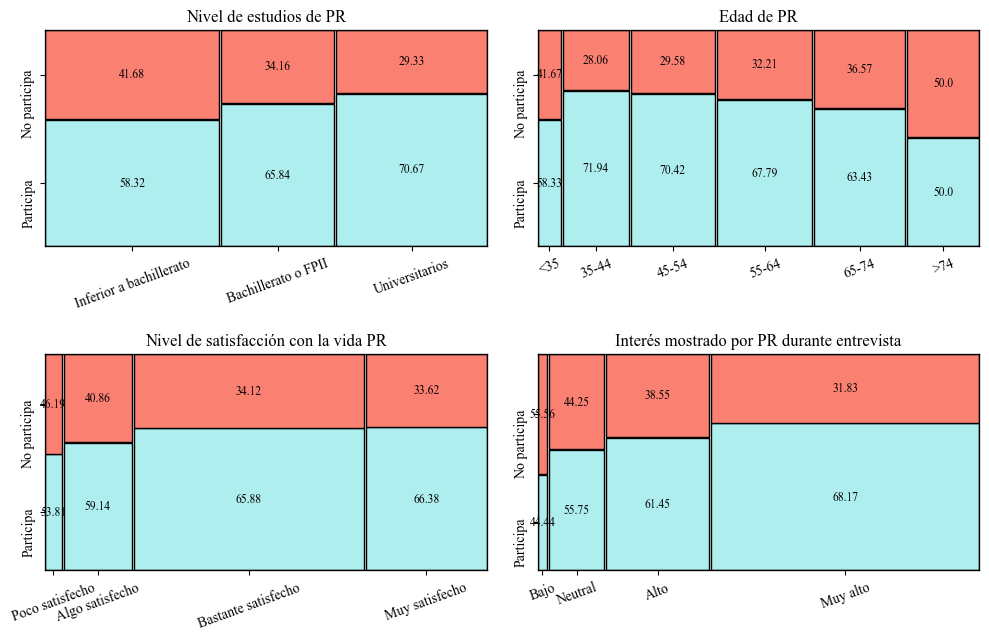
\includegraphics[width=1\textwidth]{figs/figure2.png}
	\caption{Participación en EFF2020 por características y actitudes de PR en EFF2017}
	\label{fig:fig2}
\end{figure}

La figura \ref{fig:fig2} contiene los gráficos de mekko de la participación en la EFF2020 según el nivel máximo de estudios alcanzados de la PR, su edad y su satisfacción con la vida en 2017 y el interés que mostró durante la entrevista de la EFF2017. El gráfico superior izquierdo muestra que la proporción de hogares que no participó en la EFF2020 es mayor cuanto menor era el nivel de estudios de la PR en 2017. Una posible explicación de este resultado podría deberse a la menor tenencia de productos financieros por parte de hogares de menor nivel educativo (\cite{hospido2023encuesta}). El cuestionario de la EFF contiene muchas preguntas sobre muchos productos financieros diferentes, y es razonable pensar que alguien que no posee este tipo de activos piense que no tiene sentido participar en esta encuesta. Un entrevistador con este conocimiento podría preparar un argumentario orientado a destacar que sin su participación no se podría identificar a hogares con sus características y así para poder diseñar políticas económicas específicas para esos hogares.

En el gráfico superior derecho se ve que la proporción de hogares que participó en 2020 aumenta a medida que aumenta la edad de la PR en 2017, excepto cuando ésta tenía menos de 35 años, que presenta la segunda proporción más alta de los grupos de edad. El resultado para los hogares más jóvenes podría explicarse por el hecho de que cada vez menos de estos hogares son propietarios de su vivienda principal (\cite{eff2014results}, \cite{eff2017results}, \cite{eff2020results}) y esto puede hacer que sean más propensos a mudarse, y por tanto ser más difíciles de localizar. El caso de las PR de mayor edad podría explicarse por motivos de fallecimiento.

Finalmente, en los gráficos de la parte inferior de la figura \ref{fig:fig2} vemos, por un lado, que la proporción de hogar que dejan de participar en 2020 se reduce a medida aumenta el nivel de satisfacción con la vida de la PR en 2017, y por otro, que la proporción de hogares que participaron en 2020 aumenta a medida que aumenta el interés por la encuesta. Este último resultado es razonable y útil de saber para el entrevistador porque puede basar su argumentario para convencer al hogar en ese interés.

\subsection*{Características hogar}

En este apartado se analiza a nivel exploratorio la posible relación que puedan tener las características del hogar con el panel attrition. En concreto, se analizan las variables de renta, riqueza y tenencia de deudas. La renta y la riqueza son el eje central de la EFF y es habitual incluirlas de alguna manera en cualquier análisis que se haga con los datos de la encuesta.

En la figura \ref{fig:fig3} hay tres gráficos de mekko en el que se observa la proporción de hogares que participaron en la EFF2020 según la posición relativa de cada hogar en las distribuciones de renta anual y riqueza bruta\footnote{La riqueza bruta se define como la suma del valor de todos los activos que posee el hogar (activos reales + activos financieros = riqueza bruta).} de los hogares españoles en 2017, y también si el hogar tenía deudas pendientes en 2017. La posición relativa de cada hogar dentro de la distribución de renta se muestra indicando los percentiles de la distribución total entre los que se sitúa cada hogar. Si el nivel de renta de un hogar lo sitúa entre los percentiles 60 y 80 del total de la renta de hogares en España, entonces ese hogar está en la categoría "P60-P80" de la distribución de renta, y si se sitúa por encima del percentil 90, la categoría es "\verb|>|P90".

\begin{figure}[ht]
	\centering
	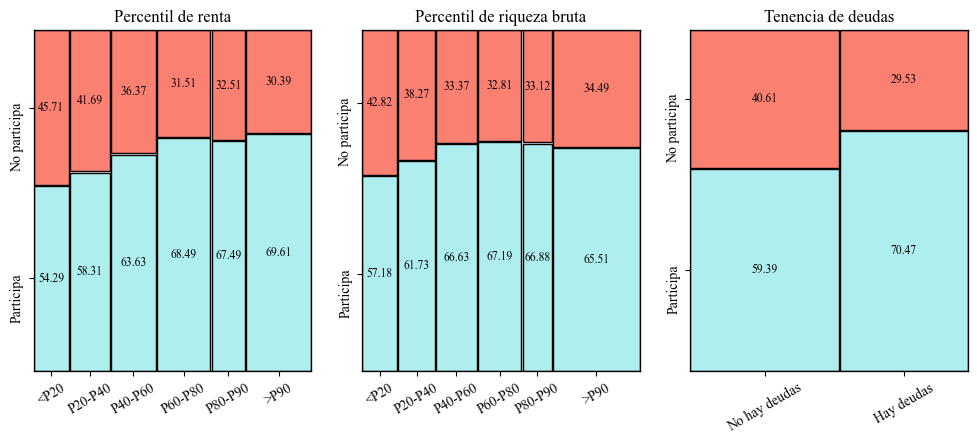
\includegraphics[width=1\textwidth]{figs/figure3.png}
	\caption{Participación en EFF2020 por renta, riqueza y tenencia de deudas en EFF2017}
	\label{fig:fig3}
\end{figure}

En el gráfico de la izquierda de la figura \ref{fig:fig3} se observan dos tendencias diferentes dependiendo del nivel de renta anual de 2017. Por encima del percentil 60 no se aprecian grandes diferencias en la proporción de panelistas que no participaron en 2020, pero por debajo de ese percentil se ve que la proporción de hogares que no participaron es mayor cuanto menor es el nivel de renta. Una posible explicación puede venir de que los niveles de tenencia de activos son menores cuanto menor es el nivel de renta de los hogares (\cite{eff2017results}) y, como se ha comentado para el nivel educativo, es razonable pensar que un hogar que tiene pocos activos considere que no tiene sentido participar en una encuesta como la EFF. Estas dos tendencias también se observan para la distribución de riqueza bruta, pero en este caso la tendencia se observa por debajo del percentil 40 de riqueza bruta. La explicación de por qué la proporción de abandonos es mayor sería similar a la de renta. Si no se tienen activos, se puede pensar que no tiene sentido participar en la EFF.

Finalmente, el gráfico de la derecha muestra la proporción de hogares que participaron en la EFF2020 según si tenían deudas pendientes en 2017. Se observa que la proporción de hogares que no participan en 2020 es mayor entre los hogares que no tenían  deudas en 2017.

\subsection*{Duración de las entrevistas}
\label{subsection:duration}

En esta última pieza de análisis exploratorio se comenta el tratamiento de valores atípicos detectados en la duración de las entrevistas. En el entrenamiento de los modelos de la sección \ref{section:evaluation_models} se ha utilizado la duración total de la entrevista en segundos. Este valor se obtiene del fichero paradata calculando, para cada hogar, la suma de los segundos que pasaron en cada pantalla del CAPI durante la entrevista. Al analizar la distribución de las duraciones se encontraron valores atípicos que indicaban que hubo entrevistas que duraron más de 20 horas, cuando las entrevistas suelen durar entre una hora y hora y media (\cite{effmethod2017}).

\begin{figure}[ht]
	\centering
	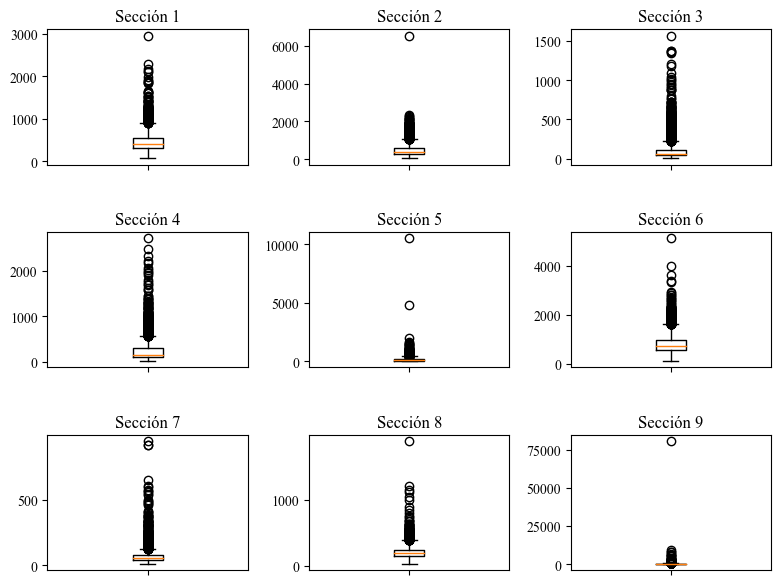
\includegraphics[width=1\textwidth]{figs/figure4.png}
	\caption{Duración por sección del cuestionario en la EFF2017}
	\label{fig:fig4}
\end{figure}

A partir de la información en el fichero paradata se calcularon las duraciones de cada una de las nueve secciones de la EFF. La figura \ref{fig:fig4} contiene los gráficos box-plot de las duraciones de las 9 secciones del cuestionario de la EFF2017. En estos gráficos se ve que hay valores atípicos en todas las secciones, y que algunos son particularmente altos, especialmente en la sección 9. Se sospecha que los entrevistadores no cerraron bien la aplicación del ordenador o la tablet al tomar un descanso, o al interrumpir una entrevista, o al terminarla.

Estos valores tan altos representan un error de medición importante que puede afectar a los modelos de predicción, por lo que es necesario tratarlos. Como hay secciones que contienen más preguntas que otras, la duración en cada sección dependerá de cuántas preguntas se formulen en cada sección. Como el fichero paradata contiene esa información, se decide imputar la duración a nivel de sección, y en concreto se imputan los valores que estén por encima del percentil 99.9 de la duración de dicha sección. Se utiliza el algoritmo kNN (\textit{k-nearest neighbors}) con k=5 y distancia euclídea. Como rasgos de cada sección se calculan el número de preguntas que se formulan una sola vez, el número total de preguntas formuladas, el número de veces que se vuelve a una pantalla anterior, el número de paradas, el número de preguntas categóricas con 1-4 opciones de respuesta, 5-9 opciones de respuesta o más de diez opciones de respuesta, y el tiempo pasado en preguntas monetarias. Tras la imputación, se calcula la duración total de la entrevista como la suma de las duraciones de todas las secciones. Este procedimiento se implementa por separado para las duraciones de cada ola.

\section{Evaluación de modelos}
\label{section:evaluation_models}

\subsection*{Rendimiento de los modelos sobre el conjunto de test}
El cuadro \ref{table:test} contiene los resultados de la evaluación de los modelos entrenados con algoritmos de machine learning con respecto al modelo de referencia de Regresión Logística Logit. Recordemos que los modelos se han entrenado con datos de la EFF2017 para predecir la no participación de los hogares panelistas en la EFF2020. El ejercicio del test consistía en predecir la participación de los hogares panel en la ola EFF2022 utilizando información de la EFF2020.

Las métricas de evaluación que se utilizan son Accuracy, Precision, Recall, F1 y ROC AUC. La métrica de referencia que utilizada para la evaluación es la ROC AUC, que se encuentra en la parte derecha del cuadro. Esta métrica mide el rendimiento entre la tasa de falsos positivos y falsos negativos. Toma valores de 0.5 a 1, con 1 siendo un predictor perfecto, y 0.5 el que se obtendría con una estimación realizada de manera aleatoria.

\begin{table}[ht]
    \centering
    \begin{tabular}{lccccc}
    \hline
        \textbf{Modelo} & \textbf{Accuracy} & \textbf{Precision} & \textbf{Recall} & \textbf{F1} & \textbf{ROC AUC} \\ \hline
        Logit & 0,6556 & 0,3749 & 0,3573 & 0,3659 & 0,5959 \\ 
        CART & 0,6434 & 0,3338 & 0,2835 & 0,3066 & 0,5521 \\ 
        Random Forest & 0,6489 & 0,3529 & 0,3148 & 0,3328 & 0,5821 \\ 
        XGBooster & 0,6718 & 0,3772 & 0,2769 & 0,3194 & 0,5911 \\ 
        Naive Bayes & 0,6254 & 0,3504 & 0,4063 & 0,3763 & 0,5798 \\ \hline
    \end{tabular}
    \caption{Métricas de evaluación de los modelos de predicción en el conjunto de test}
    \label{table:test}
\end{table}

El modelo de referencia de este estudio, el Logit, presenta una ROC AUC de 0,5959. Se considera que un valor inferior a 0,6 es un resultado malo, por lo que el modelo Logit no es un buen predictor. Con respecto a los otros modelos, observamos que el CART y el Naïve Bayes presentan valores más bajos que el Logit, de 0,5521 y 0,5798 respectivamente. El Random Forest y el XGBooster, en cambio, presentan valores de 0,5821 y 0,5911 respectivalente, que son ligeramente superiores al del modelo Logit.

De estos resultados indican que los modelos de Random Forest y XGBooster mejoran al modelo Logit. Y entre estos dos, el Random Forest presenta valores un poco más altos en Accuracy y en Precision, y el XGBooster es mejor en Recall y F1. Pero es necesario recalcar que el valor de ROC AUC sigue estando por debajo de 0,6, por lo que, aunque se mejore el rendimiento con respecto al modelo Logit, los resultados de los test son malos.

\subsection*{¿Por qué el rendimiento de los modelos es malo?}

Los resultados de la evaluación de los modelos con el conjunto de test indican que hay modelos de machine learning que mejoran en rendimiento de la predicción con respecto a un Logit. Sin embargo, la métrica ROC AUC obtenida por el mejor modelo, el XGBOOST, señala que el rendimiento de este modelo es malo. ¿Por qué los modelos no hacen bien la predicción?

Una posible causa puede ser el overfitting, es decir, que los modelos han aprendido demasiado de los datos con los que han sido entrenados y no son capaces de generalizar bien cuando se enfrentan a datos nuevos. Si esta fuese la principal razón, lo esperable sería que su rendimiento fuese bueno si se hace el ejercicio de predicción sobre los datos de entrenamiento. Los resultados del ejercicio de predicción sobre los datos de entrenamiento pueden verse en el cuadro \ref{table:train}.

\begin{table}[ht]
    \centering
    \begin{tabular}{lccccc}
    \hline
        \textbf{Modelo} & \textbf{Accuracy} & \textbf{Precision} & \textbf{Recall} & \textbf{F1} & \textbf{ROC AUC} \\ \hline
        Logit & 0,6389 & 0,4905 & 0,4518 & 0,4704 & 0,6517 \\ 
        CART & 0,6126 & 0,4594 & 0,5178 & 0,4868 & 0,6188 \\ 
        Random Forest & 0,6596 & 0,5223 & 0,4770 & 0,4986 & 0,6726 \\ 
        XGBooster & 0,6544 & 0,5144 & 0,4675 & 0,4898 & 0,6722 \\ 
        Naive Bayes & 0,6251 & 0,4741 & 0,5178 & 0,4950 & 0,6435 \\ \hline
    \end{tabular}
    \caption{Métricas de evaluación de los modelos de predicción en el conjunto de entrenamiento}
    \label{table:train}
\end{table}

Como era de esperar, las métricas del rendimiento de las predicciones de todos los modelos sobre los datos de entrenamiento son mejores que los obtenidos en el ejercicio de test. En este caso, el modelo que presenta mejor rendimiento es el Random Forest, con una métrica de ROC AUC de 0,6726, ligeramente superior a la del XGBooster. El resto de métricas del Ranfom Forest también son ligeramente mejores que las del XGBooster. Sin embargo, esta métrica de ROC AUC está entre 0,6 y 0,75, que lo clasifica como un predictor regular. Este resultado descarta que el overfitting para explicar el mal rendimiento de los modelos, e invita a considerar otras alternativas e incluso nuevos enfoques. Estas opciones se comentan con más detalle en el capítulo \ref{chapter:conclusiones}.

\subsection*{Importancia de las variables en la predicción}

Tal y como se comentó en la sección \ref{section:method}, una ventaja de los modelos basados en árboles de decisión es que pueden ser interpretados. En el caso del Radom Forest, es posible consultar qué variables han tenido más peso a la hora de clasificar la participación de los hogares. Aunque los resultados de la predicción del training no sean buenos, merece la pena echarle un ojo por los patrones que haya podido detectar. El cuadro \ref{table:importance} presenta las 20 variables con más importancia en el modelo de Random Forest ordenadas por valor de importancia.

\begin{table}[ht]
    \centering
    \begin{tabular}{lc}
    \hline
        \textbf{Variable} & \textbf{Importancia} \\ \hline
        PR es panel & 0,0822 \\ 
        Interés PR & 0,0790 \\ 
        Razones para colaborar - Relevancia de la encuesta & 0,0605 \\ 
        Proporción de preguntas monetarias respondidas (incluye intervalos) & 0,0594 \\ 
        Posee al menos un vehículo & 0,0539 \\ 
        Tiene deudas pendientes & 0,0496 \\ 
        Situación laboral - Asalariado & 0,0475 \\ 
        Razones colaborar - Interesado en estos estudios & 0,0380 \\ 
        Posee planes de pensiones & 0,0353 \\ 
        PR consiente grabar la entrevista & 0,0348 \\ 
        Hijos viven en el hogar & 0,0318 \\ 
        Nivel educativo PR & 0,0313 \\ 
        Número de olas en las que ha participado el hogar & 0,0304 \\ 
        Sexo de PR & 0,0291 \\ 
        Número de adultos con trabajo & 0,0277 \\ 
        Posee fondos de inversión & 0,0206 \\ 
        Nivel de comprensión de las preguntas por PR & 0,0206 \\ 
        Proporción de preguntas monetarias respondidas en valor puntual & 0,0198 \\ 
        Razones para colaborar - El estudio lo lleva el BdE & 0,0195 \\ 
        Estado Civil - Casada & 0,0190 \\ \hline
    \end{tabular}
    \caption{Importancia de las variables en el modelo de Random Forest}
    \label{table:importance}
\end{table}

La importancia de una variable en el Random Forest mide el peso relativo que ha tenido una variable concreta a la hora de crear las ramificaciones de los diferentes árboles de decisiones que va generando el Random Forest durante su entrenamiento. En la participación en la EFF2020, las tres variables que más importancia tuvieron fueron que la PR fuera panel, que la PR mostrase interés durante la entrevista, y que el entrevitador indicase que el hogar colaboró por la relevancia de la encuesta. También es interesante destacar la importancia de proporción de preguntas monetarias respondidas por el hogar (incluyendo intervalos), y algunas variables que hemos mencionado en la sección \ref{section:exploring}, como son si la PR consintió que se grabase la entrevista, el nivel educativo de la PR y el número de olas en las que el hogar ha participado.
\chapter{Conclusiones y futuras líneas de trabajo}
\label{chapter:conclusiones}

En este Trabajo de Final de Master se ha intentado aplicar la implementación de \cite{beste2023case} para predecir la no participación de hogares panel en encuestas longitudinales en olas futuras al caso de la Encuesta Financiera de las Familias. Para ello, se ha usado un modelo de Regresión Logística como referencia, y se han entrenado modelos CART, Random Forest, XGBooster y Naïve Bayes. El conjunto de predictores está formado por variables que potencialmente pueden explicar la participación de un hogar en la edición siguiente de la encuesta, como por ejemplo el interés mostrado por la persona que respondió a la encuesta, el nivel de recelo que mostró durante la entrevista, su nivel de salud o si consintió que la entrevista fuese grabada.

Los modelos de Random Forest y XGBooster presentaron mejores rendimientos que el modelo de referencia Logit en todas las métricas de evaluación consideradas, pero el valor de ROC AUC del mejor de los modelos no superó el valor de 0.6, lo cual lo clasifica como un predictor malo. Para intentar aprender sobre cómo se ha hecho la predicción, se hizo el ejercicio de usar los mismos modelos para hacer la predicción con el conjunto de entrenamiento. El modelo que funcionó mejor fue el Random Forest, pero su ROC AUC no superó el valor de 0,7, que lo clasifica como un predictor regular. Al observar las variables que más importancia tuvieron durante el entrenamiento del Random Forest destabacan que la persona que contestó a la estrevista a ya formase parte del hogar desde al menos dos ediciones antes, el valor del interés que mostró también era importante, y que el entrevistador considerase que el hogar participó por la relevancia de la encuesta.

A partir de los resultados que se han visto en este proyecto, se plantean las siguientes reflexiones y los posibles pasos que se podrían dar en el futuro para este proyecto:

\begin{enumerate}
    \item La exploración de los datos sugiere que las variables seleccionadas para entrenar los modelos de predicción guardan cierta relación con la variable de attrition. Pero no son suficientes para predecir bien si un hogar panel dejará de participar en la ola siguiente. Tal y como hemos comentado al principio de este capítulo, la EFF genera una gran cantidad de variables, y se hizo un filtrado inicial basado en las implementaciones de \cite{beste2023case} y \cite{kern2021predicting}. Es posible que haya \textbf{variables que no se han incluido, y que tengan poder para predecir el attrition}. Una vía de trabajo para el futuro es \textbf{volver a revisar toda la información disponible y plantear una nueva selección de variables}. El uso de métodos de machine learning para selección de variables es una opción que se podría implementar.
    \item Las olas de la EFF seleccionadas para el estudio son las de los años 2017, 2020 y 2022 porque son las que tienen mayor cantidad de datos y también los de mayor calidad. Todos los modelos entrenados buscan utilizar datos de lo que había en 2017 para predecir algo que iba a ocurrir en 2020, que es el año en el que tuvo lugar la crisis del \textbf{Covid-19}. Y posteriormente, en el test, se utiliza información recogida durante 2020 para predecir lo ocurrido en el año 2022, cuando el mundo estaba ya superando la crisis del Covid-19. El año 2020 fue un año especial en la EFF porque seguramente mucha gente fuera más reticente a participar por el covid, lo cual afectaría a la variable target del entrenamiento). También se tuvo que cambiar la metodología de la entrevista, pasando de entrevista personal a entrevista telefónica, que afecta a la calidad de los datos (\cite{lynn2018tackling}), y por tanto a los datos de los predictores usados en el test. Ante esta problemática, se plantean dos posibles alternativas:
    \begin{enumerate}
        \item Las olas de \textbf{EFF2002 a EFF2017 son homogéneas} en lo que a metodología se refiere. Todas las entrevistas fueron personales, y no hubo una crisis como la del Covid-19. Una alternativa interesante sería crear \textbf{nuevos modelos de predicción}, pero utilizando sólo la información disponible en esas olas. Serían \textbf{menos variables} (las respuestas de los hogares y la información recogida por los entrevistadores), pero podría ser que el rendimiento fuese mejor.
        \item La EFF va a continuar realizándose en los próximos años, y con una frecuencia bienal. Se puede volver a \textbf{plantear esta misma metodología dentro unos años, utilizando sólo ediciones completadas después de 2020}, y con el beneficio de recoger toda la información que se ha estado recogiendo en las últimas ediciones y que no está disponible para antes de 2017.
    \end{enumerate}
    \item Los resultados de las predicciones sobre los datos de entrenamiento también podría explicarse por la \textbf{existencia de información no observable en el momento de hacer la predicción, y que además tenga más peso para determinar el resultado de la participación que la información recabada durante la ola anterior}. El Covid-19 es un buen ejemplo de algo que no se puede prever, pero otra cosa que también se desconoce es qué entrevistadores habrá durante la siguiente edición. En todas las ediciones hay entrevistadores nuevos, y algunos funcionan muy bien, y otros no. Tal y como comentan \cite{lynn2018tackling} y \cite{groves2006nonresponse}, el papel del entrevistador es importante para la colaboración de los hogares y la calidad de los datos. Esto puede investigarse identificando a los hogares para los que no se han hecho buenas predicciones, y analizar por un lado cómo son las características que tienen en la ola anterior, y por otro la información que se tenga sobre la ola que se intenta predecir, y comprobar si las variables que tienen más peso para explicar la participación son las de la ola corriente o las de la ola anterior.
    \item Una opción que siempre hay que considerar es un \textbf{cambio de enfoque}. Hay dos alternativas que son interesantes:
    \begin{enumerate}
        \item En la exploración de los datos vimos que los hogares que han participado sólo en una edición muestran más proporción de abandonos que los que han participado más de dos años. Una posible explicación de esto es que los hogares que han participado más de una vez están más comprometidos con el estudio, y seguramente merezca la pena \textbf{enfocar el análisis en la predicción de la participación de los paneles en su segunda ola} en vez de hacer la predicción para todos los hogares.
        \item En vez de predecir un resultado binario, de participar o no participar, se puede plantear hacer un ejercicio de \textbf{análisis de superviviencia} (survival analysis), e intentar predecir el número de ediciones en las que participará un hogar de la EFF antes de abandonar el estudio. Esta información está disponible y se podría utilizar información de todas las olas de la EFF.
    \end{enumerate}
\end{enumerate}


% bibliografia
\addcontentsline{toc}{chapter}{Bibliografía}
\bibliographystyle{apalike}
\bibliography{referencias}

\end{document}